\documentclass[a4paper,notitlepage]{article}

\usepackage[top=2cm, bottom=2cm, left=3cm, right=3cm]{geometry}

\usepackage{amssymb, amsmath}
\newtheorem{mydef}{Definition}

\usepackage{boxedminipage}
% This needs to occur before hyperref and minted
\usepackage{float}

\usepackage[usenames,dvipsnames]{xcolor}

\usepackage{multirow}

\usepackage[hyphens]{url}
\usepackage{hyperref}

\usepackage{appendix}
\usepackage[numbers]{natbib}

\usepackage{graphicx, subfigure}
\usepackage{epstopdf}

\usepackage{tabularx}
\usepackage{longtable}

\usepackage{dirtree}

\usepackage{comment}

\usepackage[firstpage]{draftwatermark}
\SetWatermarkText{\includegraphics[width=\paperwidth,angle=-45]{Images/wallpaper}}

% Use minted and set the visual style to be the
% same as the one used by visual studio
\usepackage{minted}
\usemintedstyle{vs}

% Allows use of autoref with lables in listings
\providecommand*{\listingautorefname}{Listing}

\usepackage{caption}

\newcommand{\mysideways}[1]{\begin{sideways}#1\end{sideways}}

\usepackage[parfill]{parskip}
\setlength{\parindent}{0pt}
\setlength{\parskip}{0.75\baselineskip}

% A better tilde (~)
\newcommand{\mytilde}{\raise.17ex\hbox{$\scriptstyle\mathtt{\sim}$} }

% For distributed algorithms
\newcommand{\res}[1]{\mbox{\textbf{#1}}}% for reserved words
\newcommand{\qq}{\qquad}% for spacing
\newcommand{\assign}{\mathrel{:=}}% for assigning variables
\newcommand{\var}[1]{\mbox{\emph{#1}}}% for variables

% For use in the title page
\newcommand{\HRule}{\rule{\linewidth}{0.5mm}}

% Predicate language syntax highlighting
\usepackage{listings}
\definecolor{keywordblue}{RGB}{20,105,176}
\lstdefinelanguage{Hoppy}{
    morekeywords=[1]{all,function,as,returning,in,using},
    morekeywords=[2]{this},
    morekeywords=[3]{int,float},
    morekeywords=[4]{Neighbours,abs,mean,max,min,sum,len},
    sensitive=true,
}
\lstset{
    language=Hoppy,
    keywordstyle=[1]\color{keywordblue},
    keywordstyle=[2]\color{OliveGreen},
    keywordstyle=[3]\color{YellowOrange},
    keywordstyle=[4]\color{Purple},
    basicstyle=\ttfamily,
    columns=fullflexible,
}

\lstdefinelanguage{Dragon}{
    morekeywords=[1]{IPUSH,IPOP,IFETCH,ISTORE,IADD,ISUB,IMUL,IDIV1,IDIV2,IINC,IDEC,IEQ,INEQ,ILT,ILEQ,IGT,IGEQ,IABS,IVAR,ICASTF},
    morekeywords=[2]{FPUSH,FPOP,FFETCH,FSTORE,FADD,FSUB,FMUL,FDIV1,FDIV2,FEQ,FNEQ,FLT,FLEQ,FGT,FGEQ,FABS,FVAR,FCASTI},
    morekeywords=[3]{AFETCH,ALEN,ASUM,AMEAN,AMAX,AMIN},
    morekeywords=[4]{HALT,CALL,JMP,JZ,JNZ},
    morekeywords=[5]{VIINC,VIDEC,VIFAFC,THISC},
    morekeywords=[6]{AND,OR,XOR,EQUIVALENT,IMPLIES,NOT},
    morecomment=[l]{//},
    sensitive=true,
}
\lstset{
    language=Dragon,
    keywordstyle=[1]\color{Cyan},
    keywordstyle=[2]\color{WildStrawberry},
    keywordstyle=[3]\color{YellowOrange},
    keywordstyle=[4]\color{Violet},
    keywordstyle=[5]\color{ForestGreen},
    keywordstyle=[6]\color{BurntOrange},
    basicstyle=\ttfamily,
    columns=fullflexible,
}

\newcommand{\sourcecode}[3]{%
\inputminted[linenos=true,tabsize=4,fontsize=\small,frame=lines,framesep=2mm]{c}{#1/#2}
\inputminted[linenos=true,tabsize=4,fontsize=\small,frame=lines,framesep=2mm]{c}{#1/#3}
}


% For \begin{acknowledgements}
% From: http://www.latex-community.org/forum/viewtopic.php?f=47&t=5464
\makeatletter
\newcommand\ackname{Acknowledgements}
\if@titlepage
  \newenvironment{acknowledgements}{%
      \titlepage
      \null\vfil
      \@beginparpenalty\@lowpenalty
      \begin{center}%
        \bfseries \ackname
        \@endparpenalty\@M
      \end{center}}%
     {\par\vfil\null\endtitlepage}
\else
  \newenvironment{acknowledgements}{%
      \if@twocolumn
        \section*{\abstractname}%
      \else
        \small
        \begin{center}%
          {\bfseries \ackname\vspace{-.5em}\vspace{\z@}}%
        \end{center}%
        \quotation
      \fi}
      {\if@twocolumn\else\endquotation\fi}
\fi
\makeatother


% From: http://nepsweb.co.uk/docs/bnf.pdf
% For writing predicate language productions
\newcommand{\pn}[1]{\langle \textnormal{#1} \rangle}
\newcommand{\pp}{\models}
\newcommand{\oo}{\; \mid \;}
\newcommand{\sk}{\dots }
\newcommand{\ww}{\;}
\newcommand{\nn}{\perp}
\newcommand{\sm}[1]{\textnormal{#1}}
\newcommand{\sd}[1]{\textnormal{\it #1}}

\newcommand{\smlst}[1]{\textnormal{\lstinline[language=Hoppy]|#1|}}

\begin{document}

\begin{titlepage}
\begin{center}

% Upper part of the page
\includegraphics[scale=0.6]{the_warwick_uni_blue.eps}\\[0.75cm]

\textsc{\LARGE \bfseries Department of Computer Science}\\[1.5cm] 

\textsc{\Large \bfseries Fourth Year Project}\\[0.5cm]

% Title
\HRule \\[0.4cm]
{\Huge \bfseries Towards Practical Debugging of Wireless Sensor Network Applications}\\[0.4cm]

\HRule \\[9.5cm]

\vfill
\vfill
\vfill
\vfill

% Author and supervisor
\noindent{
\begin{minipage}{0.4\textwidth}
\begin{flushleft} \large
\emph{Authors:}\\
Matthew Bradbury (0921660) \\
Tim Law (0918647) \\
Ivan Leong (0830934) \\
Daniel Robertson (0910210) \\
Amit Shah (0904778) \\
Joe Yarnall (0905247)\\
\end{flushleft}
\end{minipage}}
\hfill
\noindent{
\begin{minipage}{0.4\textwidth}
\begin{flushright} \large
\emph{Supervisor:} \\
Dr.~Arshad Jhumka
\end{flushright}
\end{minipage}}

\vfill
\vfill
\vfill
\vfill
\vfill

% Bottom of the page
{\large October 2012 - July 2013}

\end{center}
\end{titlepage}

%No numbering on first and second pages
\pagestyle{empty}
\thispagestyle{empty}\clearpage

\newpage

\begin{abstract}
Debugging tools are vital for developers to produce reliable software, however traditional tools are less useful when developing software for new system paradigms such as wireless sensor networks. As wireless sensor networks (WSNs) become increasing prevalent in our lives it will become ever more important that the software they are running works reliably and to do this debugging tools will be required. This project investigates how predicates can be specified and accurately checked throughout WSNs and how errors can be reported to a base station. We also develop a system that facilitates reporting predicate statuses to a desktop application.
\newline
\newline
\noindent \textbf{Keywords} - Wireless Sensor Networks; Debugging; Reliability; Predicate Checking;
\end{abstract}

%\begin{acknowledgements}
%Acknowledgements
%\end{acknowledgements}

\clearpage


\pagestyle{plain}
\setcounter{page}{1}

\tableofcontents
\clearpage

% !TeX root = Report.tex
\section{Introduction}

\subsection{What is a Wireless Sensor Network?}

A wireless sensor network, or WSN for short, is a collection of networked sensors called Motes; these sensors are capable of short range wireless communication and they have the ability to sense their surrounding environment\cite{Mica2002,TankBible}. The network forms a distributed system that can perform a variety of distributed algorithms, usually data gathering and similar tasks. To communicate, each node is equipped with a radio that allows them to send and receive messages to neighbouring nodes within a limited range. To sense the environment motes typically have a range of embedded sensors such as heat, light, humidity and many others. They typically contain a simple central processing unit (CPU), which is programmed to control the hardware on the motes. The CPU also processes events which are triggered by the hardware (such as messages being sent and received) and it also handles any other computation necessary for the operation of the system. As the platform is designed to be mobile the motes do not operate on a mains power supply, instead they run off stored energy in a battery. WSNs is a field of Computer Science that is currently the focus of much research and wireless sensor networks have a wide range of practical applications that stretch from battlefield intelligence for the military\cite{Akyildiz2002393,1368897,1457970} to industrial process monitoring for manufacturing companies\cite{?}.

A defining characteristic of designing applications for wireless sensor networks is the restricted and finite energy supply available to each node. Therefore, wireless sensor nodes tend not to use expensive broadcasting protocols such as IEEE 802.11 \cite{Mica2002}, but instead use much simpler alternatives to save energy. For example wireless protocols such as IEEE 802.15.4 ZigBee \cite{1253873, 4014617} are designed to be used by wireless sensor networks and have a lower energy usage associated with them. Some applications rely on even lower level behaviour specified by a certain MAC layer \cite{5751321,4469515,Polastre:2004:VLP:1031495.1031508,1019408,Buettner:2006:XSP:1182807.1182838}, these applications involve a trade-off between development time and energy usage. Where simplicity is often sacrificed for decreased energy usage. Using these simple protocols unfortunately has the downside of meaning that broadcasts are subject to several types of collisions and message losses. So it is very important that the software running on the nodes is designed to handle these cases. Being battery powered means that development of applications for Wireless Sensor Networks is fundamentally limited to maximising the system's lifetime so that the highest utility can be achieved from the network.

As wireless sensor nodes operate in harsh outdoors condition\cite{SzewczykPMC04, Werner-Allen:2006:FYV:1298455.1298491}, there is a high probability of them failing. These faults can range from hardware damage caused by environmental conditions or tampering, software bugs, or simply a denial of service caused by nodes running out of power. So algorithms and software need to be designed to handle these potential failures, otherwise they risk catastrophic failure when they encounter these issues.

Wireless sensor nodes are designed with the intention for them to operate in remote and traditionally unreachable locations with no human input for the lifetime of their operation\cite{1437066}. Given this a defining characteristic of a WSN system is that any applications developed for it must be self-configuring in nature; this is, the system must be able to organize itself and the network with no external input\cite{1368897}. Evidently, solutions to this issue are often considered hand in hand with the problem of network robustness and fault tolerance.   

While a limited energy source, self-configuration and network robustness are the predominant characteristic of a wireless sensor node, there are numerous other traits or issues that can be considered. For instance it is possible for these nodes to be mobile (for example an ad-hoc network of PDAs or motes built into soldiers helmets) \cite{4224091}, this can lead to very interesting behaviour in handling communication between these nodes.

%TODO: MORE OBSCURE WSN BEHAVIOUR CONSIDERATIONS

\subsection{The Problem - Debugging Distributed Systems}

Developing a distributed system is considered a particularly challenging task, more so than a traditional application, there are several reasons for this. Firstly, Within a distributed system multiple processes must execute in parallel, this means that variables may be updated independently or in repose to other processes which can lead to a myriad of synchronisation and timing issues that the developer must account for. Secondly, traditional programming languages are not well suited to develop distributed programs\cite{93692,345131}.

In any system, software or otherwise, developed by humans there is the potential for mistakes. Mistakes can be benign or they can cause unintended behaviour and system failures. Developing tools to detect these \emph{bugs} and notify the developer so they can be corrected is an incredibly important part of any toolchain. For example the GNU toolchain has utilities such as gdb\cite{?}, this allows developers to place breakpoints in code which will halt the programs execution at that state so that it can be examined. There are also numerous other tools that look for memory issues (valgrind\cite{Bond:2007:TBA:1297105.1297057,Nethercote:2007:SBM:1254810.1254820,seward2004valgrind}), security flaws (TOOL NAME\cite{?}) and many other classes of bugs.

Developing distributed systems is a difficult task; however, debugging these systems can be even more challenging\cite{345131}. When considering a distributed system if you want to examine the state of a system at a given point you cannot simply set a breakpoint in your local binary. The solution to this debugging is non-trivial, this is due to the difficulties that arise from distributed systems being non-deterministic in nature due to message communications \cite{1676929,Joyce:1987:MDS:13677.22723,Fagerstrom:1988:DTD:55823.55833}. Be it when the message started transmission, how long it took, if it succeeded or in what order transmissions occurred. So every time a distributed program is run it is possible for a different result to be obtained, due to the different order of execution. This goes against one of the usual assumptions of debugging traditional applications where it is assumed that one execution with a set of inputs will execute in exactly the same way again with the same set of inputs \cite{?} (i.e. determinism).

As the execution may be different each time in a distributed system it is not suitable to wait for a bug to occur, and then try to work out where it is. Rather, the system needs to be self-evaluating its state as it executes the distributed program; if a fault is detected, then the debugging tools will report the issue. One way to do this it to test if the system satisfies some global predicate, of which there has been much work to find and check different classes of these predicates \cite{553309,345831,277788}. However, of all the work that has been done, little of it has focused on wireless sensor networks where an important focus is perhaps the trade-off between accuracy and the report-ability of a predicate with the aim of reducing energy usage. In this paper we will discuss our development of just such a set of tools, we intend to focus on developing a system that can accurately evaluate predicates and provide useful information about real sensor networks running outside of a simulator.

\subsection{Related Work}

\subsubsection{Fault-Error-Failure Cycle}
%TODO: Joe: Needs Work

It should be clear that the types of predicates are important to consider when developing a predicate checking mechanism. Also important are the types of errors that these predicate checking algorithms can detect. To understand this it is first important to understand how errors can arise, which can be done by examining the fault-error-failure cycle. This cycle says that a \emph{fault} once caused by either some external influence (e.g. radiation leading to bit-flips in memory \cite{1017791}) or internal influence (e.g. code bugs) will lead to an \emph{error}, this is the \emph{activation} step. An error is the manifestation of the fault (e.g. memory holding the incorrect value). An error then leads to a \emph{failure} in the step called \emph{propagation}, the failure of the system is an observable deviation from the system's specification (e.g. allowing doors to be opened that should remain closed). It is not always the case the faults lead to errors, or errors lead to failures, sometimes multiple faults or errors are respectively required to cause a single error or failure. \cite{1335465}

There is a choice of what should be measured and checked in predicates; should faults, errors or failures be measured? Faults cannot be measured \cite{?} in a way that is possible for a mote, so they are discounted. That leaves measuring errors and failures. Typically failures would be the event being measured \cite{?} as that is what arises after an error actually causes the issue to happen. However, errors can also be measured if there is a dedicated program checking the state and comparing it to an expected state \cite{?}. For example an ECC (error correcting code) such as a Hamming Code can be used to detect and correct an error (in this case a bit-flip) in some memory after a fault (such as a voltage surge ) \cite{hamming1950error}.

Much of what has been discussed has involved transient faults such as those caused by environmental conditions, however, there is a class of faults that are a lot more common and much easier to resolve - faults caused by software bugs. These faults can lead to programs ending up in the wrong state and performing incorrectly. There has been a certain amount of work that looks into detecting traditional distributed system bugs (such as deadlock \cite{5587352,5284172}) in wireless sensor networks. However, there has been little work in looking into providing tools to aid in system debugging.

\subsubsection{Classes of Distributed Predicates}
%TODO: Joe: Needs Work

To begin with it is important to understand what predicates are relevant to distributed systems. First off we have a distinction between global and local predicates, global predicates involve taking a consistent global snapshot of the system and checking whether the snapshot satisfies the global predicate \cite{277788} and local predicates instead work with a subset of the network \cite{553309}. These predicates have also have a notion of stability, a stable predicate will remain true once it has turned true (e.g. termination), whereas unstable predicates can alternate between true and false. Finally there is a distinction between weak and strong, where a weak predicate holds if there exists an observation where the predicate is true and a strong predicate holds if it is true for all observers of the distributed computation\cite{553309,Cooper:1991:CDG:127695.122774}. Knowing what classes of predicates there are is important because when checking certain properties of a system a certain class of predicate will be required and thus a certain implementation will be needed to ensure the predicate is correctly checked. An example of this is when running an algorithm using global snapshots to detect stable predicates, that same application may not be suitable to detect unstable predicates because the predicate could switch to false and then back to true before the next snapshot.

\subsubsection{Existing Sensor Network Predicate Checking Tools}

There are a number of existing predicate checking solutions that have already been developed that are more practical focused than the aforementioned theoretical work into global predicate detection.

\paragraph{H-SEND} One of these solutions is H-SEND \cite{herbert2007adaptive}, which stands for Hierachichal SEnsor Network Debugging. H-SEND is a framework for detecting faults in sensor networks, it was designed to minimise energy consumption and be capable of handling very large networks. As part of the implementation developer must specify invariants within their code using a custom grammar, these invariants are then semi--automatically inserted during compilation. If an invariant is violated at runtime actions are taken (such as increased logging frequency, or an error message to the base station), using these responses developer can use the information to fix the software, which possibly include uploading a patched version of the firmware.

Of the invariants that can be specified, there are typically three different dichotomies: (i) Local vs. Multi--node, (ii) Stateless vs. Stateful and (iii) Compile--time vs. Run--time. The first indicates whether the predicate needs information about the node it is being evaluated on (Local) or other nodes in the network (Multi). The second is if the invariant depends on the node's execution state (Stateful) or if it doesn't (Stateless). The third indicates if the invariant involves values that are fixed at compile time (such as integer constants) or if it compares against values obtained during run-time (such as neighbouring states or previous states).

H-SEND is optimised for WSNs in a variety of ways. For example, it minimises overhead by buffering messages it needs to send, and piggybacking them on the existing network traffic. Due to the hierarchical nature of the protocol, multinode-invariants can be checked efficiently at the closest parent node with all the required information.

\paragraph{Sympathy} One of the projects that is summarised by H-SEND's authors \citeauthor{herbert2007adaptive} in \cite{herbert2007adaptive} is a method for identifying and localizing failures called Sympathy \cite{ramanathan2005sympathy}. Sympathy is intended to be run either in pre- or post-deployment environments where it collects data from distributed nodes at a sink. When insufficient data is received it is taken to imply that there exists a problem (insufficient data is component defined). The idea is that by monitoring data (both actively and passively) between components the system can identify what kind of failure occurred in a certain area of the network. Both of which are very useful when trying to debug a failure.

It does, however, have some downsides. The first is that there is assumed to be no traffic and thus no application traffic or network congestion. These are real issues especially when applying this kind of debugging to a high throughput sensor network. There are also a number of spurious failure notification, which the authors are working on reducing, by applying a Bayes engine.

\paragraph{DAIKON} Following Sympathy's attempts to implement a Bayes engine to allow learning to better help classify response messages, there has been work on being able to automatically detect invariants in a system. DAIKON \cite{daikon} is a system that uses execution traces to produce a list of likely invariants by way of automatically inferring the invariants through the use of a prototype invariant detector.

The set of dynamically detected invariants depend on observed values and the invariants are an indication of the quality of a test suite. Daikon consists of two parts; a language specific front end and a language independent interference engine. The former executes the running program and accesses its runtime state to get the required information (consist of variables and their value). This information contains a subset of relevant variables and only these are written to the trace file. A variable is considered as relevant depending on the type of invariants targeted and whether they are accessible at an instrumentation point. This forms an input to the second part of the system - the invariant inference engine - which uses machine learning techniques and produces a set of detected invariants for the program.

The main challenge with these techniques is deducing the relevance of the invariants as it depends on the programmer's experience and knowledge of the underlying system. However, these can be improved with techniques like exploiting unused polymorphism and suppressing invariants that are logically implied by other invariants. DAIKON does not require the programmer to specify invariants for the application, however, it is not designed for distributed or resource-constrained systems like WSN.

\paragraph{DIDUCE} One of the issues with DAIKON is that it only detects possible invariants, DIDUCE \cite{diduce} (Dynamic Invariant Detection $\cup$ Checking Engine (DIDUCE)) uses a similar metholody to detect the invariants, but it also evaluates them as they are detected. Machine learning is employed to dynamically generate hypotheses of invariants for a system at run-time. The invariants begin extremely strict, and are relaxed over time to allow for new correct behaviour. The machine learning aspect means that developers do not have to specify invariants themselves (as compared to H-SEND), which proves beneficial as accurately pinpointing the values necessary for fault-free operation is non-trivial \cite{?}. DIDUCE checks against the invariants continually during a program's operation and reports all violations detected at the end of the run, whereas DAIKON merely presents the user with invariants found. For all its apparent usefulness, unfortunately DIDUCE was designed for large, complex systems rather than lightweight distributed systems with constrained resources such as sensor networks.

\paragraph{NodeMD} An alternative to debugging compared to either specifying a predicate or an invariant, or using machine learning to learn what to check for is to instead look for the faults that arise after a failure has occurred. This is the approach that NodeMD \cite{NodeMD} takes, that by looking for the faults that can cause undesired behaviour bugs in the system can be identified. NodeMD supports checking a number of fault classes: stack overflow, livelock, deadlock and application-specific faults. By having an extensible framework, developers of a system can write their own fault detectors and plug them into NodeMD's framework. The authors of NodeMD point out that ``human interaction is often the only reliable way to address many software issues'', therefore, NodeMD supports recording events that occur to humans can analyse them to find out how a failure occurred. To optimise this format for sensor network, the event are stored in a custom binary format to save space and reduce the number of messages to transmit it (if it is possible to transmit).

NodeMD also has support for a number of useful features to aid in debugging, the first is a debug mode that is entered when a fault is detected. The debug mode freezes critical parts of the system to prevent the fault from leading to errors. This prevents events such as a context switch after a stack overflow that would end up being performed incorrectly. The debug mode also resets certain OS components to a safe state, so that some components (such as the radio) are usable to report the fault that was detected.

The other two useful features are support for remote debugging and an implementation of dynamic reprogramming algorithms to update the firmware across the network. The remote debugging feature allows a human to access all the available fault information of a sensor node. Parameters can be changed to expose more information when the node is queried and the potentially useful feature of telling the node to restart is also available. Overall NodeMD provides lots of insight into the low level failures in wireless sensor networks.


\subsubsection{Practical Sensor Network Deployments}


\subsubsection{Tools and Platforms}


\clearpage

%% !TeX root = Report.tex
\section{Literature Review}

\subsection{Routing in Sensor Networks}

\subsubsection{Flooding}



\subsection{Simulating Sensor Networks}

\subsubsection{TinyOS}

\subsubsection{Contiki}
% Cite basically all the papers at: http://www.contiki-os.org/support.html

\subsubsection{NS2}

\subsubsection{JProwler}

\subsubsection{Simulating Energy Consumption}
\cite{Shnayder04}


\subsection{Sensor Network Platforms}

\subsubsection{MICA}
\cite{Mica2002}

\subsubsection{Sky}


\subsection{Practical Experience in Sensor Networks}

\subsubsection{Air Pollution}
\cite{libeliumAirPollution}
\cite{wsnpollution} Claimed: Ivan

Air pollution has been a growing concern in congested urban cities as a result of industrilization and heavy transporation. These concerns include poor air quality and visibilty and long term damaging of human health. Traditional methods of air quality monitoring involving quality control stations are expensive and provides low resolution sensing since monitoring stations are less densly deployed. Wireless sensor networks can be used as an urban monitoring system as it has the advantages of being small, easy to set up and inexpensive with real time monitoring capabilities. Sensors which have the ability to measure a wide range of meteorological data such as rainfall, wind speed, temperature, humidity and concentration of pollutants can be deployed in areas of high population density of vehicles and indistrial areas. Collected data is transmitted back to the base station via a global system for mobile communication.

Engineers from the University of Luxembourg implemented a system based on a Wireless Mesh Network of sensors to measure air pollution in Sub-Saharan African cities. These cities experience the most problems due to the increase of industry, domestic waste and fuel combustion and that many chemical industries have been established in the central urban areas. However, with poor infrastructure and telecommunication links in Africa, it would be difficult to deploy a sensor network that will measure air pollution since some pollution ares are out of range of the communication service. David Et Al. proposed a Wireless Mesh Network to establish Internet connectivty and simultaneously measure air pollution is such areas.

\subsubsection{Forest Fires}
\cite{libeliumForestFires}
\cite{FireWxNet}

\subsubsection{Great Duck Island}
\cite{SzewczykPMC04}

\subsubsection{Volcano Monitoring}
\cite{Werner-Allen:2006:FYV:1298455.1298491} Claimed: Ivan

Active volcanoes need to be monitored to predict the likihood of future eruptions so that early-warning signs can be issued for the evacuation of habitants near the volcano. Today, volcanoists use wired arrays of sensors such as seismometers and acoutic microphones to collect seismic and infrared (low-frequency acoustic) signals and determining a wide range of factors such as sources of volcanic eruptions, interior structure of a volcano and differentiating eruption signals from noise. A typical study can indlue the placement of several stations around the volcano where each contains a low distribution of wired sensors that collects data to a hard drive. Data is then collected manually in a possibly inconvenient location.

To address the issue of high power consumption of these wired sensors, Werner-Allen Et Al. \cite{?} introducted the deployment of embeddded wireless sensor networks consisting of low-power nodes with minimum CPU, memory and wireless communication capabilities. This allows for long distance real time monitoring of volcanic activities and reducing the need for manual data collection. The main challenge however is that environmental monitoring studies sample at a frequency which is much lower than the sample rate of volcanic timeseries. This is due to the limited radio bandwidth of the sensors thus requiring the need for efficient power management techniques and accurate time synchronization of the nodes. 

Werner-Allen Et Al implemented a wireless sensor network that was deployed on the Volcan Tungurahua in central Ecuador using a Mica2 sensor mote plateform and three infrasonic microphone nodes. These nodes transmitted data to an aggregation node, which relayed the data over a 9km wireless link to the base station. Time synchronization for the infrasonic sensors was done using a GPS receiver which receives a GPS time signal and relays the data 
to the infrasound and aggregator nodes. Over a period of time, the temperature and battery voltage may change and this may affect the sampling rate of the individual nodes and the precision of the time recorded from the GPS timestamp message. These uncertainties was addressed by applying a linear regression to the logged data stream giving an estimation of the node outputs. In addition, the sensor nodes where required to be protected against harsh environemnts such as rain and long exposure of sunlight by using waterproof pelican cases and 1/4-wave whip antennas.

Their first deployment on the volcano included a small network where nodes could send continuous signals to each other, however this was not feasible for a larger network deployed over longer periods of time. To solve the issue with bandwidth and energy consumption, the team implemented a distributed event detector which only transmits well-correlated signlas to the base station. A local event detection algorithm is used to trigger data collection for uncorrelated signals.

\begin{itemize}
\item Distributed Event Detector

To measure the correlated signal, the distributed detector uses a decentralized voting system among a group of nodes. Each nodes samples data at a continuous rate of 102.4Hz and buffers a window of such data while running a local event detection algorithm. If an event is triggered it uses a local radio broadcast to broadcast a vote to other nodes and a global flood to initiate globbal data collection from all the nodes. Radio contention is reduced using a token-bases scheme for sceduling transmission, where each nodes transmits their buffer one after the other. 

\item Local Event Detector

The team implemented two local event detectors; a threshold-based detector and an exponentially weighted moving average (EWMA)-based detector. The former is triggered when the signal rises above an upper threshold and below a lower threshold. However due to spurous signals such as wind noise, the detector may be suceptible to false trigger. On the other hand, the EWMA detector calculates two moving averages with different gain parameters and is triggered if the ratio of the two averages and the new sample exceeds some threshold T. This method is less affected by node sensitivity and any duplicate triggers over a window of 100 samples are suppressed.
\end{itemize}

Data collection and performance

During the deployment, the team managed to log 54 hours of continuous data which includes seismoacoustic signals from several hundred events. The raw data was used to analyse the system's performance and many challenges where discovered in the early observations. They discovered that on average only 61 percent of data was retrieved from the network and on several occasions the modems which transmitted data back to the station would experience short dropouts, causing all data aggragated from the nodes to be lost. In addition, duplicate packets were also recorded as a likely result of redundant retransmission and lost acklowledgement. Both lost and duplicate data had to be accounted for before being stored in the timebase.

Conclusion and improvements

In general, the event-triggered model was successful in detecting eruptions and other volcanic events and was able to verify the working of the local and global event detectors by examining the downloaded data. However, since the experiment was deployed over a limited area space of the volcano, further work is to be done to instrument volcanos at a larger scale. This includes, and most importantly, the management of energy and bandwidth usage of the sensors and increasing its computational power to deviate from continuous data collection to enabling the collection of well-correlated signals. 

\subsubsection{Structural Monitoring}
\cite{5508230}

\subsubsection{Development of Applications}
\cite{Fagerstrom:1988:DTD:55823.55833}


\subsubsection{Power Considerations}


\subsection{Predicates}

Before we can consider what predicates we can try to check for, or how we should check those predicates, we first need to understand what we are detecting and why. In dependable systems we need to consider the fault-error-failure cycle. This cycle says that a \emph{fault} once caused by either some external influence (e.g. radiation leading to bit-flips in memory \cite{?}) or internal influence (e.g. code bugs) will lead to an \emph{error}, this is the \emph{activation} step. An error is the manifestation of the fault (e.g. memory holding the incorrect value). An error then leads to a \emph{failure} in the step called \emph{propagation}, the failure of the system is an observable deviation from the system's specification (e.g. allowing doors to be opened that should remain closed). It is not always the case the faults lead to errors, or errors lead to failures, sometimes multiple faults or errors are respectively required to cause a single error or failure. \cite{1335465}

There is a choice of what should be measured and checked in predicates, should faults, errors or failures be measured? \textbf{TODO}


\subsubsection{GPD}

\cite{345831}
\cite{277788}
\cite{553309}


\subsection{Predicate Detection in Distributed Systems}

\subsubsection{NodeMD}
\cite{NodeMD}


\subsubsection{Sympathy}

One of the projects that is summarised by \citeauthor{herbert2007adaptive} in \cite{herbert2007adaptive} is a method for identifying and localizing failures called Sympathy \cite{ramanathan2005sympathy}. Sympathy is intended to be run either in pre- or post-deployment environments where it collects data from distributed nodes at a sink. When insufficient data is received it is taken to imply that there exists a problem (insufficient data is component defined). The idea is that by monitoring data (both actively and passively) between components the system can identify what kind of failure occurred in a certain area of the network. Both of which are very useful when trying to debug a failure.

It does, however, have some downsides. The first is that there is assumed to be no traffic and thus no application traffic or network congestion. These are real issues especially when applying this kind of debugging to a high throughput sensor network. There are also a number of spurious failure notification, which the authors are working on reducing, by applying a Bayes engine.

\subsection {DICAS: Detection, Diagnosis and Isolation of Control Attacks in Sensor Networks}

Detection, Diagnosis and Isolation of Control Attacks in Sensor Networks (DICAS) \cite{dicaspaper} is a lightweight distributed protocol for Wireless Sensor Networks that mitigates the effects of a wide-range of control traffic attacks. DICAS does this by utilizing a unique property of a wireless sensor network, this is that each node is able to monitor a part of their neighbours network traffic. Using DICAS the authors were able to create LSR a lightweight secure routing algorithm for Wireless Sensor Networks.

In DICAS nodes maintain a data structure of their first hop neighbours for local monitoring to detect malicious nodes and in local response to isolate these nodes. When a node is deployed it finds and authenticates all of its 1 hop neighbours using a pairwise shared key. These neighbours communicate their neighbours, 2 hop neighbours to the original node, and their own commitment key, which is generated using a random seed, to the newly deployed node. Each node will then have knowledge of all of its 1 hop neighbours as well as their commitment keys and all of its 2 hop neighbours.

Using this knowledge the DICAS protocol can enact a collaborative detection strategy where every node monitors the traffic going in and out of it's neighbours. Each node that is within transmission range of both the sending(X) and receiving(A) nodes of a packet are considered guard nodes of A over the link from X to A. These nodes maintain a watch buffer of packets sent from X to A, the duration and information stored are determined by the attack type under consideration by the system. Each guard node maintains a malicious counter for each link it is monitoring, if A drops, delays, changes or fabricates a packet from X then the guard node will increase its malicious counter. If the malicious counter exceeds a predefined threshold the node is considered to be malicious and is removed from the neighbours list. The guard node propagates this knowledge to all the other nodes in its neighbour list. When another node receives enough authenticated alerts about the malicious node it is excluded from its neighbours list. Once all 1 hop nodes have excluded the malicious node then it is effectively isolated from the system and all packets from or to that node are ignored.      

The authors tested the DICAS algorithm against 5 sets of attacks, these are:
\begin{enumerate}

\item Route Traffic Manipulation

\item ID Spoofing and Sybil Attacks

\item Wormhole Attacks

\item Sinkhole

\item Rushing Attack

\end{enumerate}

Additionally, the paper describes a cost analysis on the DICAS algorithm, these are the results: 
\begin{itemize}
\item Memory Overhead

The memory overhead is the most pressing of the overheads created by the DICAS algorithm. The algorithm must store several data structures on each node: a neighbours list, a watch buffer, a commitment key list and the alert list. These structures are variable on sizes dependent on the number of nodes in the network, the network layout and the MAC layer delay for acquiring a channel. Any implementation must consider the memory cost of the algorithm seriously.

\item Computation Overhead

With regards to computation they found that each packet received or sent required: one lookup for the current source and destination in the neighbour list, for an incoming packet - adding an entry to the watch buffer or for an outgoing packet - deleting an entry from the watch buffer. Since the size of the watch buffer and the neighbour list structure are relatively small, the computation time required for these operations is negligible.

\item Bandwith Overhead

When considering bandwidth the overhead was primarily gained in 2 conditions: after node deployment when a node is populating its neighbour list and during a wormhole attack detection where a node is informing its neighbours of the malicious node. However, these cases make up a negligible fraction of the total network traffic over the lifetime of a wireless sensor network.
\end{itemize}

\subsection{H-SEND: Hierachichal SEnsor Network Debugging}

H-SEND is a framework for detecting faults in WSNs, designed to minimise energy consumption. It differs from related algorithms by being capable of handling very large WSNs. \cite{?}

There are 4 main steps involved in H-SEND:

\begin{enumerate}
	\item Developer specifies invariants when writing the software
	\item Invariant checking code is (semi--)automatically inserted during compilation
	\item If an invariant is violated at runtime, actions are taken (such as increased logging frequency, or an error message to the base station)
	\item Developer can use the information to fix the software, and then upload the patched version
\end{enumerate}

There are a variety of different types of invariants that can be specified, typically characterised by the following three dichotomies:

\begin{itemize}
	\item Local vs. Multi--node invariants
	
	Invariants dependent on state on a single node are called local, as they don't require and messaging to check. If the state of multiple nodes is required for checking, the invariant is said to be multi--node.

	\item Stateless vs. Stateful invariants
	
	An invariant is stateless is it doesn't depend on a node's execution state, and stateful otherwise.

	\item Compile--time vs. Run--time invariants

	Compile--time invariants are those involving comparisons against values that do not change, whereas runtime invariants are more flexible. Runtime invariants can compare against spatial and temporal trends ---  the state of surrounding nodes, and previous states respectively.
\end{itemize}

A grammar is specified which can be used to insert invariants into source code. Existential and universal quantifiers are supported.

H-SEND is optimised for WSNs in a variety of ways. For example, it minimises overhead by buffering messages it needs to send, and piggybacking them on the existing network traffic. Due to the hierarchical nature of the protocol, multinode-invariants can be checked efficiently at the closest parent node with all the required information.

\subsubsection*{Dynamic Invariant Detection $\cup$ Checking Engine (DIDUCE)}

DIDUCE \cite{diduce} is a tool which employs machine learning to dynamically generate hypotheses of invariants for a system at run-time; the invariants begin extremely strict, and are relaxed over time to allow for new correct behaviour. The machine learning aspect means that developers do not have to specify invariants themselves, which proves beneficial as accurately pinpointing the values necessary for fault-free operation is non-trivial. DIDUCE checks against the invariants continually during a program's operation and reports all violations detected at the end of the run, whereas Daicon merely presents the user with invariants found. For all its apparent usefulness, unfortunately DIDUCE was designed for large, complex systems rather than lightweight distributed systems with constrained resources (i.e. WSNs), so it is likely to prove infeasible to use this tool for GPD.

\subsubsection*{DAIKON: A tool for dynamically detecting invariants in sensor network applications}

One method of automatically inferring invariants in applications is the use of a prototype invariant detector, DAIKON \cite{daikon}, which uses execution traces to produce a list of likely invariants. The set of dynamically detected invariants depend on observed values and the invariants are an indication of the quality of a test suite. Daikon consists of two parts; a language specific front end and a language independent interference engine. The former executes the running program and accesses its runtime state to get the required information (consist of variables and their value). This information contains a subset of relevant variables and only these are written to the trace file. A variable is considered as relevant depending on the type of invariants targeted and whether they are accessible at an instrumentation point. This forms an input to the second part of the system - the invariant inference engine - which uses machine learning techniques and produces a set of detected invariants for the program.

The main challenge with these techniques is deducing the relevance of the invariants as it depends on the programmer's expereience and knowledge of the underlying system. However, these can be improved with techniques like exploiting unused polymorphism and suppressing invariants that are logically implied by other invariants. Daikon does not require the programmer to specify invariants for the application, however, including DIDUCE, it is not designed for distributed or resource-constrained systems like WSN.


\begin{comment}
\subsection{Quality of Service}
The area of Quality of Service (QoS) within Wireless Sensor Networks (WSN) is largely unexplored, due to the large differences between WSNs and traditional wireless networks. Traditional networks determine QoS based on high bandwidth allowance, as a result of high multimedia demands of applications. WSNs typically do not need to transfer this amount of data, and have a much lower bandwidth because of this. WSNs also have a wide range of different applications, and as a result, it is not clear how to develop transferable approaches to QoS  \cite{Akyildiz2002393}. 

QoS can be reduced to 'a set of service requirements to be met when transporting a packet stream from the source to its destination' \cite{Crawley98aframework}. With traditional networks, redundancy is often introduced to allow for high load/traffic, however redundancy in WSNs can often mean wasted energy usage which is often the main QoS measure in many protocols \cite{AkkayaYounis2003}.

Akyildiz et. al. \cite{Akyildiz2002393} suggested that QoS could be measured in two ways Application and Network. The Application defines measures such as coverage, number of active sensors and exposure, while the Network is concerned with delivering the QoS constrained data, while maintaining network efficiency (minimising resources).

Akyildiz et. al. further went on to describe the challenges specific to WSN; 
\begin{itemize}  
			\item Resource Constraints - Battery life, memory, bandwidth etc
			\item Unbalanced traffic - Traffic flows from large set of sensors into a small set of sink nodes
			\item Data redundancy - The re-transmission of data could result in wasted energy usage
			\item Network Dynamics - Failing nodes/wireless links, energy conservation, mobility etc
			\item Scalability 
			\item Multiple sink nodes - Each node could have a different set of requirements
			\item Packet Critically - Some data may need to flow through the network quicker than other pieces
			\item Multiple traffic types - Different pieces of data flowing through the network at the same time
\end{itemize}

QoS is a difficult term to define, mainly due to its various meanings and perspectives, because of this, measurements of quality must be generated based on the application involved, and the specific requirements of that application.


\subsection{MAC Protocols}

\subsubsection*{Energy-efficient MAC Protocol Designed for WSN for IoT (The submarine paper)}

\cite{6128220} discusses the energy efficiency of existing protocols, including the original adaptation of MAC for WSNs - Sensor MAC (SMAC). Describes the operation of SMAC, which uses a fixed listen/sleep cycle to reduce idle listening time and thus save energy. Goes on to mention two improvements on SMAC: first Timeout MAC (TMAC), in which the listen/sleep cycle is adapted according to network traffic, by means of a simple timeout mechanism; then $\mu$-MAC, which alters between contention and contention-free periods. The former is used to establish network topology and initialise sub-channels (collections of time slots), which are used in the contention-free period to transmit without collisions.

The authors then propose a power-controlled MAC protocol (PC-MAC), which determines the required transmission power level for a packet, thus aiming to save unnecessary energy usage when sending over short distances. This calculation assumes the physical layer of the nodes can transmit frames at one of a discrete set of power levels notified by the MAC layer. Once calculated, the minimum required power for each of a node's neighbours is stored in that node's Schedule and Power Level Table, an extension of the Schedule Table used for synchronising sleep cycles in SMAC. The protocol preserves the collision- and overhearing-avoidance properties of SMAC.
Authors report energy savings of between 50\% and 96\% for average node distances ranging from 10m down to 1m. These findings were generated solely using simulations, but assuming they hold for a hardware WSN the benefits for energy efficiency are significant enough to warrant serious consideration.


\subsubsection*{Energy Analysis of Four WSN MAC Protocols}

Four power-aware protocols based on the MAC framework implemented in TinyOS on TelosB motes and were tested using broadcast, convergecast and local gossip traffic patterns \cite{5751321}. Motivation: testing of the protocols side-by-side under controlled parameters, to rule out the innumerable extraneous factors that make direct comparison of separately-published protocols difficult.

Outlines history of power-saving MAC strategies, beginning with the duty cycles as described above in the operation of SMAC. Then describes the next development --- low-power listening (LPL), using transmission preambles and channel polling to reduce idle listening times. More advanced protocols use a hybrid of these two techniques.

Protocols tested:
\begin{enumerate}
	\item Scheduled Channel Polling MAC (SCP-MAC):
	\begin{itemize}
		\item Modification of LPL by waking up all neighbouring motes to listen at the same time. This leads to shorter preambles and duty cycles than typical LPL protocols (i.e. BMAC). However, all neighbours share a listening slot, so overhearing is common.
	\end{itemize}
	
	\item Asynchronous Schedules MAC (AS-MAC):
	\begin{itemize}
		\item Eliminates overhearing by assigning unique time slots for each mote to listen; the times when each mote wakes up to transmit/receive are determined by its internal Neighbour Table. At each wakeup, a mote polls for packet receptions, and motes transmit during a contention window overlapping with this wakeup slot. Loss of contention signals a retry during the recipient's next wakeup. AS-MAC uses sync packets and non-uniform offsets to offer unique receiver receptions slots, even in dense neighbourhoods.
	\end{itemize}
	
	\item Crankshaft:
	\begin{itemize}
		\item Similar to AS-MAC in that time is divided into frames, which are sub-divided into receiver slots. Frames include broadcast and unicast slots such that all neighbouring motes wake up for the all of the former, and only their own unicast slot. The ratio between the two types of slot is configurable at compile time, and the number of unicast slots is independent of the number of motes. As such, dense WSNs often feature multiple receivers contending for receptions during the same slot; clock synchronization in Crankshaft relies upon upper layers.
	\end{itemize}
	
	\item Broadcastable AS-MAC (BAS-MAC):
	\begin{itemize}
		\item During implementation of broadcasting in AS-MAC (using multiple unicast transmissions), it was noticed that a broadcasting mote must stay awake for the duration of every receive slot in the network; for nontrivial network sizes, this would be infeasible. As such, a separate protocol was created. BAS-MAC is based heavily on AS-MAC, but defines a broadcast interval; a time slot during which all neighbouring motes wake up simultaneously.
	\end{itemize}
\end{enumerate}

Measurement of the energy usage of each protocol was approached by recording the amount of time motes spent in each radio state, and multiplying each of these times by a constant representing the energy usage of that state per unit time. These constants were determined using an oscilloscope connected to a mote running AS-MAC (as energy consumption per state is protocol-independent). Minor alterations were made to each protocol to  ``level the playing field" in the case of slow/complex protocol initialisations and inapplicable network assumptions.

The results of the experiments, organised by network traffic type, are as follows.
\begin{enumerate}
	\item Local gossip:
	
	AS-MAC demonstrated highest energy efficiency for this traffic type, with Crankshaft and BAS-MAC both using approximately 40\% more energy (due to increased idleness caused by the lack of broadcasts), and SCP-MAC using more energy still due to its overhearing avoidance being inapplicable due to the packet-based TelosB motes.
	
	\item Convergecast:
	
	AS-MAC shows the best overall performance again, though for receiving motes the energy usage of SCP-MAC is a very close second. Again, the unused second wakeup for Crankshaft and BAS-MAC leads to idling.
	
	\item Broadcast:
	
	As AS-MAC is inherently poorly suited to broadcasts, its sender used almost triple the energy of that of the next-least efficient protocol, though its receivers were most efficient by a small margin. Thus, in a single-hop network where the base station node is not battery powered, it is a good choice. However, SCP-MAC performed best overall, by a significant margin over both Crankshaft and BAS-MAC.
\end{enumerate}

The authors conclude that no single protocol excels in all circumstances; AS-MAC and SCP-MAC are more efficient with non-broadcast and broadcast traffic, respectively, where BAS-MAC performs moderately well in each scenario. However, as the base station for our network will typically be a laptop or desktop, the disadvantage of AS-MAC in broadcasting could potentially be ignored. The authors also suggest using a framework such as MLA to host a suite of protocols suited to different tasks, each of which may be swapped in to match the current circumstances.

This last point may well prove to be beyond the scope of our project, however the results for individual protocols may prove useful. It is unfortunate that a fair comparison between these protocols and PC-MAC could not be made.

\subsubsection*{A Traffic Queue-aware MAC Protocol for WSNs}

This paper \cite{4469515} introduces the traffic Queue-aware Sensor MAC protocol (QSMAC), based on SMAC to predict amount of data traffic in a network.

After describing the operation of SMAC (as above), the authors highlights the problem of a fixed cycle duration in networks where traffic loads can fluctuate; an overflowing node buffer queue may cause packets to be discarded, causing additional energy expenditure in resending lost packets and debasing the network QoS.

The basic operation of QSMAC involves examining the average increase rate of data packets in a node's buffer queue. When this rate is more than one per second, packets are arriving faster than they can be processed using the default SMAC cycle, so the cycle duration is halved to double its effective processing speed. When the buffer is almost empty, the default cycle is restored.

Simulations show performance greater than that of SMAC in terms of packets' delay, energy consumption, packet reception ratio and network throughput. As above, if these benefits translate to real hardware, QSMAC potentially offers a real improvement over existing wireless MAC protocols. However, its use in our network will have to be carefully considered, as it is currently unknown whether fluctuating traffic loads will be a likely scenario.
\end{comment}

%\clearpage

% !TeX root = Report.tex
\section{Model}

As stated in the introduction we are investigating developing tools to aid in debugging the distributed programs running on wireless sensor networks. We aim to do this by implementing libraries that use different technique to check predicates, with a focus on correctly evaluating these predicates. In order to do this we first need to model the situation that our libraries will be used in to aid in the explanation of our findings.

To begin with we model a wireless sensor network as a graph $G = (V, E)$ where $V$ is a set of nodes. If we have two nodes $u$ and $v$ that can communicate $\{u, v\} \in E$, we assume that this communication is bi-directional. Every node in the network has a unique identifier 

\begin{mydef}
\emph{$m$-Hop Neighbourhood}: Given a node $n$ the $m$-hop neighbourhood of that node is the set of nodes that are within $m$ hops of node $n$. When we refer to this neighbourhood it will not contain the node $n$.
\end{mydef}

As we are dealing with simulators and physical hardware, there is no assumption of reliable links between nodes. Techniques will be described later on that increase the probability of a message reaching its target, but do not ensure it.

Every node in the network is assumed to have the same hardware and thus the same capabilities. As every node has the same capabilities, every node has similar properties such as: transmission range and initial power levels. We assume that the network is working in isolation to other networks and is not receiving other electromagnetic interference.

When checking predicates we much deal with the notion of the \emph{correctness of evaluation} of a predicate. As can be seen from the definition this involved the notion of time because the values used to evaluate the predicate can change over time.

\begin{mydef}
\emph{Correctly Evaluated Predicate}: A predicate $P$ is correctly evaluated at time $\tau$ if the results of evaluating that predicate with global knowledge at time $\tau$ is the same as the result of predicate $P$.
\end{mydef}

To evaluate a predicate there is some function $PE$ that takes a mapping from node identifiers to a user-defined structure of valued about that node and returns a boolean. By executing this function the result of a predicate is obtained. The input can be obtain through various means. The next chapter will discuss how this function is evaluated and how the required information can be disseminated to the node that requires it to perform the evaluation.

\subsection{Algorithm Descriptions}



\clearpage

% !TeX root = Report.tex
\section{Predicate Evaluation}

\subsection{Predicate Scripting Language}

\subsubsection{Required Features}

\begin{enumerate}
	\item Numerical support (Integer and Floating point) ($+$ $-$ $\times$ $/$ $=$ $\neq$ $<$ $\leq$ $>$ $\geq$)
	\item Set support (Creation and operating on) ($\cup$ $\cap$ $\setminus$ $\{\}$ $\forall$ $\exists$)
	\item Limited function support (eg. $Neighbourhood(N, H)$)
	\item Limited struct support (eg. $N.Temperature$)
	\item Ability to specify predicate target(s) (Single node, multiple nodes or entire network)
	\item Ability to get the current node ($this$)
	\item Ability to get sensor information on a node (temperature, humidity, \ldots)
	\item Ability to get node information (Distance to Sink, \ldots)
\end{enumerate}

\subsubsection{Non-Required Features}

There are lots of features that are usually provided by scripting languages that would cause undesirable effects such as inflating the binary size.

\begin{enumerate}
	\item Strings
	\item Complicated data structures (Lists, Arrays, Dictionaries, \ldots)
	\item Library features (Custom libraries or built-in libraries)
	\item Interactive mode (terminals)
	\item IO
\end{enumerate}


\subsubsection{Evaluation Methods}

\begin{enumerate}
	\item Send scripting language to node, they interpret and evaluate it
	\item Compile predicate on base station, compress and send to node(s) for evaluation
\end{enumerate}

\subsubsection{Scripting Languages Considered}

\begin{enumerate}
	\item eLua \url{http://www.eluaproject.net/} \cite{elua}
	\item SCript \url{http://www.sics.se/~adam/dunkels06lowoverhead.pdf} \cite{dunkels06lowoverhead}
	\item wren \url{https://github.com/darius/wren} \cite{wren}
	\item Write the predicate in C, compile it to machine code and send it to the nodes to be evaluated
	\item \url{http://dunkels.com/adam/tsiftes11database.pdf} Antelope
\end{enumerate}


\subsubsection{Getting and Waiting for Neighbourhood Data}

\begin{enumerate}
	\item If all neighbours are known then 1-hop predicates can wait for each node to send data. This has extra memory and communication requirements
	\item If we do not know who our n-hop neighbours are then we can just set a time out to wait for results
	\begin{enumerate}
		\item If we do not receive all items what should be done?
		\item Should we report that the predicate is true, even though we didn't receive all the information?
	\end{enumerate}
	\item What data should be sent from surrounding nodes and how could we access it?
\end{enumerate}



\subsection{Where to Evaluate Predicates}

Given the problem of assigning slots in a TDMA MAC protocol, one would wish to ensure that no node within two hops of any given node has the same slot. This raises a question of where this predicate should be evaluated to ensure minimum energy usage in its evaluation.

The first predicate we might consider is the one where for ever node, we get the 2-hop neighbourhood and check that none of those nodes have the same slot as the initial node. This means that we would need to send:
\begin{enumerate}
	\item A message from the base station to the node asking it to evaluate the predicate
	\item A message from the node to each of its 2-hop neighbours
	\item Each 2-hop neighbour needs to send a message back to the node
	\item The node would need to wait for its neighbours to send the messages, then evaluate the predicate. This would imply that the node would need to know who is in its two hop neighbourhood
	\item The node would need to report to the base station the result of the predicate
\end{enumerate}

So we would need at best $2\Delta_{sink} + 2|Neighbours(n, 2)|$ messages to evaluate this predicate for one node.

\begin{align}
\label{eq:2-hop-slot-pred}
& \hspace{3em}	\forall n \in Nodes \cdot \\
& \hspace{6em}		\forall n' \in Neighbours(n, 2) \cdot \\
& \hspace{9em}			(n.slot \neq n'.slot)
\end{align}


The second predicate we could consider is the one where every node checks their 1-hop neighbourhood for slot collisions. Here we model the 2-hop nature of the predicate differently, because instead of checking on the node that we want to check for slot collisions, we check on the node between two nodes that might have slot collisions.

\begin{enumerate}
	\item A message from the base station to the node adjacent to that we asking to check slot collisions
	\item A message from the node to each of its 1-hop neighbours
	\item Each 1-hop neighbour needs to send a message back to the node
	\item The node would need to wait for its neighbours to send the messages, then evaluate the predicate. This would imply that the node would need to know who is in its two hop neighbourhood
	\item The node would need to report to the base station the result of the predicate
\end{enumerate}

So we would need at best $2(\Delta_{sink} + 1) + 2|Neighbours(n, 1)|$ messages to evaluate this predicate for one node.

\begin{align}
\label{eq:1-hop-slot-pred}
&				\forall n \in Nodes \cdot \\
& \hspace{3em}		\forall n' \in Neighbours(n, 1) \cup \{n\} \cdot \\
& \hspace{6em}			\forall n'' \in Neighbours(n, 1) \cup \{n\} \cdot \\
& \hspace{9em}				(n' \not= n'' \implies n'.slot \neq n''.slot)
\end{align}

Overall we can assume that $|Neighbours(1, n)| \leq |Neighbours(2, n)|$, so checking 1-hop neighbours would in general require fewer message. Also we can assume that when checking these predicates, we would make sure that every node is checked (as the predicates are defined). This means that the first predicate would duplicate the checks: checking node $n$ for a collision with $n'$ and when $n'$ is asked to check the predicate it will query $n$.

However, if we were not asking the entire network to check for this property, then the first predicate would behave better. This is because the second predicate would have to be called for every 1-hop neighbour of the intended node. However, as it is assumed that the entire network would be asked if this predicate holds, then the second predicate is better.


\subsection{Implementing Primitives}

There are certain primitives that we are going to need to implement. One of these is the $Neighbours(n, h)$ primitive, that takes a parameter $n$ that is the node we wish to get neighbour information on and $d$ which is the distance in hops from the node $n$ that we will ask for information.

\begin{align}
\label{eq:hcluster-neighbours-predicate}
& \hspace{3em}	\forall n \in Nodes \cdot \\
& \hspace{6em}		\exists n' \in Neighbours(n, H) \cdot \\
& \hspace{9em}			IsClusterHead(n)
\end{align}

An example of a predicate that uses $Neighbours(n, h)$ is shown above. This predicate is for Hierarchical Clustering where $H$ is a parameter that defines the distance between cluster heads. The predicate checks that for every node there is a neighbour in the $H$-hop neighbourhood that is a cluster head.

An alternative way that we might specify this predicate is to check that the distance between a node and the cluster head (that it knows the address of) is within $H$ hops.

\begin{align}
\label{eq:hcluster-distance-predicate}
& \hspace{3em}	\forall n \in Nodes \cdot \\
& \hspace{6em}		IsSink(n) \lor Distance(n, ClusterHead(n)) \leq H
\end{align}

However, there is an issue with this predicate. How would we implement the $Distance(n, n')$ primitive? With $Neighbours(n, h)$ we know how far we need to ask for information ($h$ hops), with $Distance(n, n')$ the maximum distance that we will need to wait for information to return from is the diameter of the network. Unfortunately we cannot assume that the diameter is known. If instead we take a time-out approach there is no way that we can guarantee to wait for the correct amount of time. For example if we wait enough time to check if a node is at maximum $D$ hops from the given node the node will need to wait for $2 \times D \times T_{send}$ time units. However, if the node we are trying to find the distance of is at $D + 1 $ hops then we will not believe the two nodes are connected. To reliably wait to check if two nodes are connected in a network where the diameter is not known we will need to wait for $\infty$ time units. Thus making $Distance(n, n')$ impossible to implement without knowing the diameter.


\subsection{Domain Specific Language}

\subsubsection{Definition}
\begin{eqnarray*}
	\pn{eval} & \pp & [ \pn{target} ] \ww \pn{using} \\
	\pn{target} & \pp & \sm{all} \\
	~ & \oo & \pn{number}\sm{.}\pn{number} \\
%
	\pn{using} & \pp & \sm{using} \ww \sm{Neighbours}\sm{(}\pn{number}\sm{)} \ww \sm{as} \ww \pn{variable} \ww \sm{in} \ww \pn{using} \\
	~ & \oo & \pn{predicate} \\
%
	\pn{predicate} & \pp &  \sm{(}\pn{predicate}\sm{)} \\
	~ & \oo & \pn{quantifier}\sm{(}\pn{variable} \ww \sm{:} \ww \pn{variable} \ww \sm{\mytilde} \pn{predicate} \sm{)}\\
	~ & \oo &  \pn{predicate} \ww \pn{logical-binary} \ww \pn{predicate} \\
	~ & \oo &  \pn{logical-unary} \ww \pn{predicate} \\
	~ & \oo &  \pn{var-expr} \ww \pn{math-logical-binary} \ww \pn{var-expr} \\
%
	\pn{var-expr} & \pp & \sm{(}\pn{var-expr}\sm{)} \\
	~ & \oo & \pn{variable} \\
	~ & \oo & \pn{number} \\
	~ & \oo & \pn{string}\sm{(}\pn{this-variable}\sm{)} \\
	~ & \oo & \pn{var-expr} \ww \pn{math-binary} \ww \pn{var-expr} \\
	~ & \oo & \sm{abs}\sm{(}\pn{var-expr}\sm{)} \\
	~ & \oo & \pn{set-fn}\sm{(}\pn{variable}\sm{)} \\
	~ & \oo & \pn{transform-set-fn}\sm{(}\pn{transform-fn}\sm{,} \ww \pn{variable}\sm{)} \\
%
	\pn{this-variable} & \pp & \pn{variable} \oo \sm{this} \\
	\pn{variable} & \pp & \pn{string} \\
%
	\pn{transform-fn} & \pp & \pn{string} \\
	\pn{transform-set-fn} & \pp & \sm{sum} \oo  \sm{mean} \oo \sm{max} \oo \sm{min} \\
	\pn{set-fn} & \pp & \sm{len} \\
%
	\pn{logical-binary} & \pp & \sm{\&}  \oo \sm{\textbar} \oo \sm{\textasciicircum} \oo \sm{=\textgreater} \oo \sm{\textless=\textgreater} \\
	\pn{logical-unary} & \pp & \sm{!} \\
	\pn{math-logical-binary} & \pp & \sm{==} \oo \sm{!=} \oo \sm{\textless} \oo \sm{\textless=} \oo \sm{\textgreater} \oo \sm{\textgreater=} \\
	\pn{math-binary} & \pp & \sm{+} \oo \sm{-} \oo \sm{*} \oo \sm{/} \oo \sm{**} \oo \sm{\%} \\
%
%	\pn{string} & \pp & \pn{alpha}\pn{string-rest} \\
%	\pn{string-rest} & \pp & \nn \oo \pn{alpha}\pn{string-rest} \oo \pn{digit}\pn{string-rest} \\
%
%	\pn{alpha} & \pp & \sm{A}\dots\sm{Z} \oo \sm{a}\dots\sm{z} \\
%	\pn{number} & \pp & \pn{sign} \pn{number-first} \oo \pn{number-first} \\
%	\pn{number-first} & \pp & \pn{digit} \oo \sm{1}\dots\sm{9}\pn{number-rest} \\
%	\pn{number-rest} & \pp & \pn{digit} \oo \pn{digit}\pn{number-rest} \\
%	\pn{digit} & \pp & \sm{0}\dots\sm{9} \\
%	\pn{sign} & \pp & \sm{+} \oo \sm{-} \oo \nn \\
	\pn{quantifier} & \pp & \sm{@} \oo \sm{\#} \\
\end{eqnarray*}

\textbf{TODO: Add float expansions}

used \url{http://cs.lmu.edu/~ray/notes/javacc/} and \url{http://www.engr.mun.ca/~theo/Misc/exp_parsing.htm} to get infix operator parsing working

\subsubsection{Examples}

\begin{figure}[H]
\begin{verbatim}
using Neighbours(2) as twohopn in
    @(x : twohopn ~
        slot(x) != slot(this)
    )
\end{verbatim}
\caption{Check that no two neighbours have the same slot}
\end{figure}

\begin{figure}[H]
\begin{verbatim}
using Neighbours(1) as onehopn in
    @(x : onehopn ~
        @(y : onehopn ~
            addr(x) != addr(y) => slot(x) != slot(y)
        )
    )
\end{verbatim}
\caption{Check that no two neighbours have the same slot}
\end{figure}

\begin{figure}[H]
\begin{verbatim}
temperature(this) <= 40.0
\end{verbatim}
\caption{Check that our temperature is less than or equal to 40 degrees}
\end{figure}

\begin{figure}[H]
\begin{verbatim}
using Neighbours(2) as twohopn in
    abs(temperature(this) - mean(temperature, twohopn)) <= 10.0
\end{verbatim}
\caption{Check that the average neighbour temperature is with 10 degrees of ours}
\end{figure}


\begin{figure}[H]
\begin{verbatim}
using Neighbours(H(this)) as neighbours in
    #(node : neighbours ~
        ch(this) == addr(node)
    )
\end{verbatim}
\caption{Check cluster head is in H-hop neighbourhood}
\end{figure}



\begin{figure}[H]
\begin{verbatim}
using Neighbours(1) as onehopn in
    using Neighbours(2) as twohopn in
        @(a : onehopn ~
            #(b : twohopn ~ addr(a) == addr(b))
        )
\end{verbatim}
\caption{Check 1-hop neighbourhood is in 2-hop neighbourhood}
\end{figure}


\begin{figure}[H]
\begin{verbatim}
using Neighbours(1) as onehopn in
    base-station-distance(this) == min(base-station-distance, onehopn) + 1
\end{verbatim}
\caption{We are one hop further from the base station than the closest of our neighbours}
\end{figure}


\subsection{Virtual Machine}

\subsubsection{Opcodes}

\begin{verbatim}
_ is either I for int or F for float

HALT
    Halts execution

_PUSH (_)
    Pushes an _ onto the stack

_POP
    Pops the stack by sizeof(_) bytes

_FETCH (variable id - ubyte)
    Fetches the value of the given variable and pushes the
    first sizeof(_) bytes of it onto the stack

_STORE (variable id - ubyte)
    Stores the first sizeof(_) bytes in the variable
    of the given name

AFETCH (variable id - ubyte)
    Fetches the value of the array named in the parameter
    at the integer index at the top of the stack

ALEN (variable id - ubyte)
    Pushes an integer onto the stack containing the length
    of the named array
	
ASUM (variable id - ubyte) (function id - ubyte)
    Over the user defined array stored in the variable whose
    name is the first parameter, transform it using the function
    whose name is the second parameter. On this transformed data
    calculate the mean and push the result as a float onto the
    top of the stack.

CALL (function id - ubyte)
    Calls the named function on the data on top of the stack.
    The data this is called on is popped and the result
    is pushed onto the stack.

ICASTF
    Pops an integer off the stack, casts it to a float
    then stores it back on the stack

FCASTI
    Pops a float off the stack, casts it to a integer
    then stores it back on the stack

JMP (int)
    Jumps to a position in the code relative to the start
    of the program

JZ (int)
    Reads the top of the stack as an integer, if it is 0
    the program jumps to the location, otherwise evaluation
    continues

JNZ (int)
    Reads the top of the stack as an integer, if it is not 0
    the program jumps to the location, otherwise evaluation
    continues

_ADD     1 = 0 op 1
_SUB     1 = 0 op 1
_MUL     1 = 0 op 1
_DIV1    1 = 0 op 1
_DIV2    1 = 1 op 0
    Performs a mathematical operations on the first two sizeof(_)
    values on the stack. Pops both values off the stack, stores
    the result in the same type back on the stack.

IINC
    Pops the top of the stack by sizeof(int) bytes, increments
    the value as an integer. Pushes the result back on the stack

_EQ	     1 = 0 op 1
_NEQ     1 = 0 op 1
_ILT     1 = 0 op 1
_LEQ     1 = 0 op 1
_GT	     1 = 0 op 1
_GEQ     1 = 0 op 1
    Performs a mathematical operations on the first two sizeof(_)
    values on the stack. Pops both values off the stack, stores
    the result in an integer on the stack.

AND     1 = 0 op 1
OR      1 = 0 op 1
XOR	    1 = 0 op 1
    Performs a logical operation on the first two values on the
    stack. These are not bitwise operations and the expected
    formats of the values are integers. 0 is false, 1 is true.
    Pops both values off the stack,
    stores the result in an integer back on the stack.

NOT
    Pops an integer off the stack, performs logical not on it.
    Pushes the result back on the stack.
	
_VAR (variable id - ubyte)
    Creates a variable of type _ with the id set to the given
    unsigned byte.
\end{verbatim}

\clearpage

% !TeX root = Report.tex
\section{Implemented Algorithms}

\dirtree{%
.1 Common/.
.2 containers/.
.3 linked-list.[h/c].
.3 array-list.[h/c].
.3 unique-array.[h/c].
.3 map.[h/c].
.2 net/.
.3 eventupdate.[h/c].
.3 multipacket.[h/c].
.3 nhopflood.[h/c].
.3 nhopreq.[h/c].
.3 rimeaddr-helpers.[h/c].
.3 tree-aggregator.[h/c].
.2 debug-helper.[h/c].
.2 led-helper.[h/c].
.2 random-range.[h/c].
.2 sensor-converter.[h/c].
}

\subsection{Container Library}

Contiki comes with a list container \footnote{Header: \url{https://github.com/contiki-os/contiki/blob/master/core/lib/list.h} Source: \url{https://github.com/contiki-os/contiki/blob/master/core/lib/list.c}}, however, when we were developing with their linked list we found that it was awkward to use in some situations (for instance creating an array of lists) so we decided that we needed to find a better list library. Our problem was that other container libraries were unlikely to be optimised to the low memory requirements or support the special compile chain used by Contiki. So rather than waste time searching and integrating an external library we decided to write our own set of containers. By doing the main benefit we gained was that we knew how the containers worked so had a better understanding how to use them.

Another reason to develop our own containers was that we desired an list where the data was stored in an array, this was for because it provides lower memory overhead and the types of operations we would be performing (append and empty) meant that an array backed list would be better. The lower memory overhead comes from the fact that an array-based list doesn't need to store a pointer to the next element as it is implicit (due to the contiguous memory) that a pointer to the current element's pointer plus one is the next element. This means that in a list of $N$ items our singly linked list implementation will require $(\text{sizeof}(T) + \text{sizeof}(void *) \times 2) \times N$ bytes of memory, whereas our array list implementation will require $(\text{sizeof}(T) + \text{sizeof}(void *)) \times N$ bytes of memory.

Our linked list implementation uses more memory compared to Contiki's implementation because their list is \emph{intrusive}\footnote{Boost Containers: \url{http://www.boost.org/doc/libs/1\_53\_0/doc/html/intrusive/presenting\_containers.html}}. What is meant by this is that the pointer to the next item in the list is contained in the structure stored in the list \cite{?}. Meaning their list uses the same amount of memory as our array list. However, because the list is intrusive it makes it more difficult to use as the implementation detail leaks into the structure using the library, this was why developing our own non-intrusive list made it easier to develop code.

We also developed containers that helped abstract certain concepts (such as list uniqueness or accessing elements by key) to decrease code duplication and allow us to express the code in a higher-level way making implementation easier. One thing to note is that for the containers we did not focus on implementing some of their functions to the standard complexity. For example our map implementation has requires O(N) for both insert and fetching, where these may be implemented as O(1) on average (hash tables) or O(log N) (trees), however due to the requirements of low memory we decided to keep using the array as the backing store for the data with the aim to keep memory for at the expense of non-optimal container management functions. The increased time complexity should make little difference as the containers tend to have few elements in them (i.e. hundreds rather than millions, where complexity would start to be important \cite{?}).

Finally, all of these custom containers are tested by a test suite that checks for functional correctness. Also the test suite was run using \verb|valgrind|\footnote{\url{http://valgrind.org/info/tools.html}} to check for memory leaks and corruption.


\subsection{Network Library}

\subsubsection{Event Update}

\begin{figure}[H]
  \centering
  \begin{boxedminipage}{\linewidth}
    % 
    \null Process $j$ - \res{event-update}\\
    %
    \null \textbf{variables}\\
    %
    \null\qq \var{period}: timer init $P_{generate}$;\\~\\
    %
    \null\qq \% The previous node data sent to the network\\
    \null\qq \var{previous}: struct init $\bot$;\\~\\
    %
    \null \textbf{constants}\\
    %
    \null\qq \% Generate Period, how often we should check for a change in the data\\
    \null\qq \var{$P_{generate}$}: time;\\~\\
    %
    \null\qq \% Checks if the data differs\\
    \null\qq \var{differs}: function takes (struct, struct) returns boolean;\\~\\
    %
    \null\qq \% Gets the data of the current node\\
    \null\qq \var{data}: function takes () returns struct;\\~\\
    %
    \null\qq \% The probability of sending our data, even if no change occurred\\
    \null\qq \var{chance}: real;\\~\\
    %
    \null \textbf{parameters}\\
    %
    \null\qq \% The distance we need to send information\\
    \null\qq \var{distance}: int;\\~\\
    %
    \null \textbf{actions}\\
    %
    %
    \null\qq \% Check for changes\\
    \null\qq \emph{check}::~\res{timeout}(\var{period}) $\rightarrow$\\
    \null\qq\qq $\var{force} \assign \res{RandReal}(0, 1) \leq \var{chance}$;\\
    \null\qq\qq $\var{changed} \assign \var{previous} = \bot \lor \var{differs}(\var{data}(), \var{previous})$;\\
    \null\qq\qq \res{if} ($\var{force} \lor \var{changed}$) \res{then}\\
    \null\qq\qq\qq $\var{previous} \assign \var{data}()$;\\
    \null\qq\qq\qq \res{nhopflood}$\langle j, \var{previous}, \var{distance}\rangle$;\\
    \null\qq\qq \res{fi}; \\
    \null\qq\qq \res{set}($\mathit{period}$, $P_{generate}$); \\~\\
    %
    %
    \null\qq \% Receiving Change message\\
    \null\qq \emph{receive}::~\res{nhopflood.recv}$\langle source, data, hops\rangle \rightarrow$\\
    \null\qq\qq \% Prevent delivery if being told that the current node's data has changed\\
    \null\qq\qq \res{if} ($j \not= source$) \res{then} \\
    \null\qq\qq\qq \% Inform library caller of data change\\
    \null\qq\qq\qq \res{data-changed-callback}(\var{data}, \var{hops}); \\
    \null\qq\qq \res{fi}; \\
    %
    %
  \end{boxedminipage}
  \caption{Event Update Broadcast Algorithm}
\end{figure}


\subsubsection{Multi-Packet}

In Contiki sending a single packet has its limits, there is only so much data you can get in a single packet. There are two C macros that are relevant to this \verb|PACKETBUF_HDR_SIZE| which is set to 48 bytes and \verb|PACKETBUF_SIZE| which is set to 128 bytes\footnote{packetbuf.h \url{http://contiki.sourceforge.net/docs/2.6/a00302.html}}. This means that in general we will only be able to send a packet containing 128 bytes of information, but what if we have a data structure that spans 300 bytes? Then we will need to have a way to send multiple packets and a receiver that can put the packets back together in the correct way to deliver the data.

Contiki's data transfer primitives for their RIME protocols are fairly hidden because of their focus on uIPv6. We found \verb|ruldolph0| first \footnote{ruldolph0 \url{http://contiki.sourceforge.net/docs/2.6/a01735.html}} and then \verb|rucb| (Reliable Unicast Bulk Transfer) much later \footnote{rucb \url{http://contiki.sourceforge.net/docs/2.6/a00365.html}}. However, both of them have problems, the API is very convoluted and seems more geared towards sending very large files across the network. This is very different to our aim, which is to send relatively small packets of data to a specific neighbour. So we wrote our own API that would split data of any given size and reassemble it once received, our API was not focused on processing data chunks like \verb|ruldolph0| or \verb|rucb|, but simply operated on a block of memory given to it. This is a case where a simpler API made development much easier for us. Admittedly because our implementation uses dynamic memory allocation it could potentially perform worse, but because the energy of sending and receiving messages dwarfs the energy usage of the CPU, we feel that easier development tradeoff it worth it. Also, now that code has been written to use this API, the \verb|multipacket| library itself could always be rewritten to use \verb|rucb| as a base to run more efficiently.


\subsubsection{N-Hop Flood}

\subsubsection{N-Hop Request}
Contiki provides broadcast primitives to allow the flooding of messages through the network, however the \verb|trickle|\cite{Levis04trickle} primitive only allows a single source node\footnote{trickle.h \url{http://contiki.sourceforge.net/docs/2.6/a00381.html}}, which presents a problem, when multiple nodes are attempting to send a message N-hops away. 
In some cases \verb|reliable unicast| could be used to target the specific nodes for which the message is intended. This, however, is not suitable when the identifies of the nodes is not known, or in situations when storing routing tables is not appropriate. 

Our response to this was to develop a primitive which would flood the network, a fixed number of hops from the source, whilst allowing multiple nodes to use the same primitive, with different messages. Our implementation uses a \verb|stubborn broadcast| to pass the message along a chain, only rebroadcasting the message when the hop limit (the number of hops the message is intended to travel) has not been reached. If a message has been seen before by a node (and the number of hops left is lower than before) it is simply ignored and not passed on. In the case where the hop count for a 
duplicate message is higher than the previously seen count, it is then rebroadcast, so that all the intended recipients will receive the message.  
After a fixed time, messages are then sent back to the source along a chain, this time is reset whenever a message with a higher hop count is seen.  Each node stores the ID of the node that it received the message from, and the response message is sent back to that node. In turn, that node will forward the message to the node it received the original message from, eventually the message will end up at the source, to be processed.

%TODO: Note about performance maybe?
%Could also put a graphic of the chain here too

\begin{figure}[H]
  \centering
  \begin{boxedminipage}{\linewidth}
    % 
    \null Process $j$ - \verb|n-hop-req|\\
    %
    \null \textbf{parameters}\\
    %
    \null\qq \% The number of hops left to send a message\\
    \null\qq \var{hop\_limit}: int\\~\\
    %
    %
    \null \textbf{variables}\\
    %
    \null\qq \%The nodes a given message was seen from\\
    \null\qq \var{mote\_records}: map\\~\\
    %
    %
    \null \textbf{constants}\\
    %
    \null\qq \% Send Data Period, the time between receiving a request for data, and sending it\\
    \null\qq \var{$P_{send\_data}$}: time;\\~\\
    %
    %
    \null \textbf{actions}\\
    %
    %
    \null\qq \% Receiving Message\\
    \null\qq \emph{receive}::~\res{recv}$\langle source, data, hop\_count, id\rangle \rightarrow$\\
    \null\qq\qq \res{if} ($mote\_records.contains(id)$) \res{then}\\
    \null\qq\qq\qq \res{if} ($mote\_records.hop\_count(id) < hop\_count$) \res{then} \\
    \null\qq\qq\qq\qq \res{stbroadcast.send($message$,$hop\_count -1$)};\\
    \null\qq\qq\qq\qq \res{$mote\_records$.replace($id$,$hop\_count$)};\\
    \null\qq\qq\qq\qq \res{\var{$P_{send\_data}$}.restart()}\\
    \null\qq\qq\qq \res{fi;}\\
    \null\qq\qq \res{else}\\
    \null\qq\qq\qq \res{stbroadcast.send($message$,$hop\_count -1$)};\\
    \null\qq\qq\qq \res{$mote\_records$.add($id$,$data$,$source$,$hop\_count$)};\\
    \null\qq\qq\qq \res{\var{$P_{send\_data}$}.start()}\\
    \null\qq\qq \res{fi;}\\~\\
    %
    %
    \null\qq \% Sending Data\\
    \null\qq \emph{send\_data}:~\res{timeout}(\var{$P_{send\_data}$})$\rightarrow$\\
    \null\qq\qq \res{runicast.send}($j$,$mote\_records.getMote(id)$, $data$);\\~\\
    %
    %
    \null\qq \% Recieved Data\\
    \null\qq \emph{recv\_data}:~\res{runicast.recv}$\langle source, data, id\rangle \rightarrow$\\
    \null\qq\qq \res{if} ($mote\_records.getMote(id)$ == $self$) \res{then}\\
    \null\qq\qq\qq \% Process Data\\
    \null\qq\qq \res{else}\\
    \null\qq\qq\qq \res{runicast.send}($mote\_records.getMote(id)$, $data$);\\
    \null\qq\qq \res{fi;}\\
    %
    %
  \end{boxedminipage}
  \caption{N-Hop Request Algorithm}
  \label{fig:n-hop-req-algorithm}
\end{figure}

\subsubsection{Tree Aggregation}

As has been previously mentioned Tree Aggregation is a very useful technique employed in wireless sensor networks to aggregate a set of data to a single node in the network. It is very useful because of its ability to convey the same amount of data in potentially fewer messages. The algorithm works by first creating a tree structure such that nodes know of a parent node that they should unicast their messages to. Once this tree is set up the nodes (typically leaf nodes) unicast data to their parents, this can either happen when an event occurs or it can happen periodically. When a parent node receives a message it waits for a certain amount of time for more messages to arrive, every message it receives is stored and aggregated. After the time period is up the aggregated data is forwarded to its parent node. Once the data reaches the destination it is delivered to the user of the library.


The user of this library needs to implement four important functions:
\begin{enumerate}
\item[$\otimes_{agg}$] This function aggregates stored data with data message that has been received
\item[$\otimes_{own}$] This function aggregates the node's own data into the stored data
\item[$\otimes_{read}$] This function does the initial reading of data from a message and creates the local stored data
\item[$\otimes_{write}$] This function writes the local stored data back to a packet
\end{enumerate}


\begin{figure}[H]
  \centering
  \begin{boxedminipage}{\linewidth}
    % 
    \null Process $j$ - \res{tree-aggregation}\\
    %
    \null \textbf{variables}\\
    %
    \null\qq \var{parentdetect}: timer init $\bot$;\\~\\
    %
    \null\qq \var{seensetup}, \var{collecting}, \var{leaf}: bool init $False$, $False$, $True$;\\~\\
    %
    \null\qq \var{besthop}: int init $INTMAX$;\\~\\
    %
    \null\qq \var{bestparent}: address init $\bot$;\\~\\~\\
    %
    \null\qq \var{aggregation}: timer init $\bot$;\\~\\
    %
    \null\qq \var{collecting}: bool init $False$;\\~\\
    %
    \null\qq \var{stored}: struct init $\bot$;\\~\\
    %
    \null \textbf{constants}\\
    %
    \null\qq \% How long to wait for messages to aggregate before forwarding what the node has\\
    \null\qq \var{$P_{aggregation}$}: time;\\~\\
    %
    \null\qq \% How long to wait for parents to be detected\\
    \null\qq \var{$P_{parentdetect}$}: time;\\~\\
    %
    \null \textbf{parameters}\\
    %
    \null\qq \% The address of the node data should be aggregated to\\
    \null\qq \var{sink}: address;\\
    %
  \end{boxedminipage}
  \caption{Tree Aggregation Algorithm - variables}
\end{figure}

\begin{figure}[H]
  \centering
  \begin{boxedminipage}{\linewidth}
    \null \textbf{actions}\\
    %
    %
    \null\qq \% Set up tree: initialise\\
    \null\qq \emph{starup}::~\res{init} $\rightarrow$\\
    \null\qq\qq \res{bcast}$\langle j, \bot, 1\rangle$;\\~\\
    %
    %
    \null\qq \% Set up tree: receive message\\
    \null\qq \emph{receive}::~\res{recv}$\langle source, parent, hops\rangle \rightarrow$\\
    \null\qq\qq \res{if} ($j \not= sink$) \res{then} \\
    \null\qq\qq\qq \res{if} ($\lnot\var{seensetup}$) \res{then} \\
    \null\qq\qq\qq\qq $\var{seensetup} \assign True$; \\
    \null\qq\qq\qq\qq \res{set}($\mathit{parentdetect}$, $P_{parentdetect}$); \\
    \null\qq\qq\qq \res{fi}; \\
    \null\qq\qq\qq \res{if} ($\var{hops} < \var{besthop}$) \res{then} \\
    \null\qq\qq\qq\qq $\var{bestparent}, \var{besthop} \assign \var{source}, \var{hops}$; \\
    \null\qq\qq\qq \res{fi}; \\
    \null\qq\qq\qq \res{if} ($\var{leaf} \land \var{j} = \var{parent}$) \res{then} \\
    \null\qq\qq\qq\qq $\var{leaf} \assign False$; \\
    \null\qq\qq\qq \res{fi}; \\
    \null\qq\qq \res{fi}; \\~\\
    %
    %
    \null\qq \% Set up tree: finish detecting parents\\
    \null\qq \emph{check}::~\res{timeout}(\var{parentdetect}) $\rightarrow$\\
    \null\qq\qq \res{if} ($\var{besthop} = INTMAX$) \res{then} \\
    \null\qq\qq\qq \res{bcast}$\langle j, \var{bestparent}, INTMAX\rangle$;\\
    \null\qq\qq \res{else} \\
    \null\qq\qq\qq \res{bcast}$\langle j, \var{bestparent}, \var{besthop} + 1\rangle$;\\
    \null\qq\qq \res{fi}; \\
    %
    %
  \end{boxedminipage}
  \caption{Tree Aggregation Algorithm - Setting up tree}
\end{figure}


\begin{figure}[H]
  \centering
  \begin{boxedminipage}{\linewidth}
    \null \textbf{actions}\\
    %
    %
    \null\qq \% Send data function\\
    \null\qq \emph{send}::~\res{function}$\langle data\rangle \rightarrow$\\
    \null\qq\qq \res{multipacket.unicast}$\langle \var{bestparent}, data\rangle$;\\~\\
    %
    %
    \null\qq \% Set up tree: receive message\\
    \null\qq \emph{receive}::~\res{multipacket.recv}$\langle source, data\rangle \rightarrow$\\
    \null\qq\qq \res{if} ($j = sink$) \res{then} \\
    \null\qq\qq\qq $\var{stored} \assign \otimes_{read}(data)$; \\
    \null\qq\qq\qq $\var{stored} \assign \otimes_{own}(\var{stored})$; \\
    \null\qq\qq\qq $\res{deliver}(\otimes_{write}(\var{stored}))$; \\
    \null\qq\qq \res{else} \\
    \null\qq\qq\qq \res{if} ($\var{collecting}$) \res{then} \\
    \null\qq\qq\qq\qq $\var{stored} \assign \otimes_{agg}(\var{stored}, \var{data})$; \\
    \null\qq\qq\qq \res{else} \\
    \null\qq\qq\qq\qq $\var{stored} \assign \otimes_{read}(data)$; \\
    \null\qq\qq\qq\qq $\var{collecting} \assign True$; \\
    \null\qq\qq\qq\qq \res{set}($\mathit{aggregation}$, $P_{aggregation}$); \\
    \null\qq\qq\qq \res{fi}; \\
    \null\qq\qq \res{fi}; \\~\\
    %
    %
    \null\qq \% Set up tree: finish detecting parents\\
    \null\qq \emph{finishagg}::~\res{timeout}(\var{aggregation}) $\rightarrow$\\
    \null\qq\qq \res{multipacket.unicast}$\langle \var{bestparent}, \otimes_{write}(\var{stored})\rangle$;\\
    \null\qq\qq $\var{collecting} \assign False$; \\
    \null\qq\qq $\var{stored} \assign \bot$; \\
    %
    %
  \end{boxedminipage}
  \caption{Tree Aggregation Algorithm - Sending data}
\end{figure}


\begin{figure}[ht!]
\centering
\subfigure[Example Network]{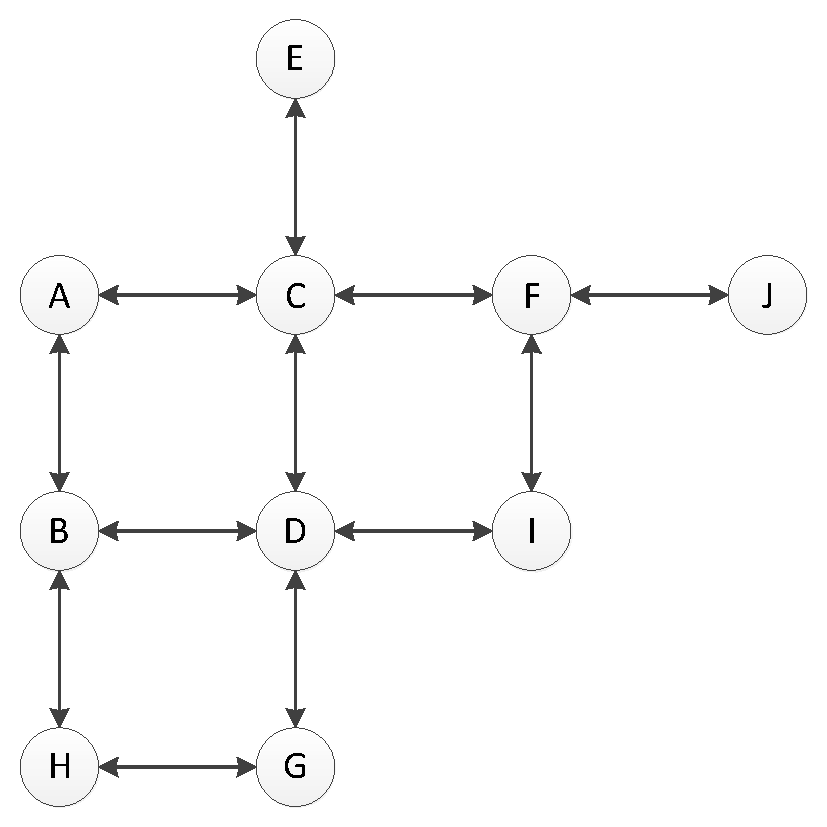
\includegraphics[width=0.5\textwidth]{Diagrams/neighbour-network}}

\subfigure[Logical Tree imposed on network]{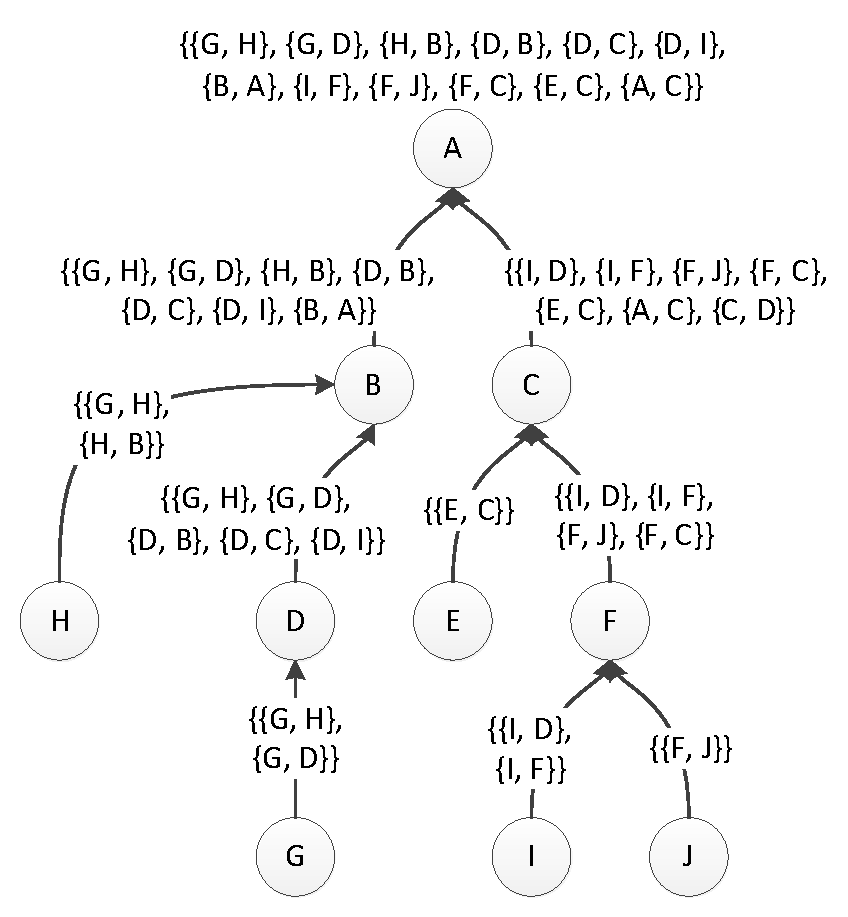
\includegraphics[width=0.5\textwidth]{Diagrams/neighbour-tree-structure}}
\end{figure}

\subsubsection{Neighbour Detect}

To aid in debugging a vital piece of information that will be required about the network is its topology. Trying to analyse network state without knowing which nodes are neighbours of other nodes, makes drawing meaningful conclusions from that data much harder. This meant that we needed a way to send neighbour information back to the sink. Thankfully part of the job is already accomplished as Contiki comes with a library to perform neighbour detection\cite{?}. We extended that library in two ways.

The first was to add more features to Contiki's neighbour detect library. As that library was very simple and supported only saying that a neighbour had been detected (with the option of providing a integer value as well). As we were aiming for this code to support changes in the network, such as nodes leaving or joining neighbourhoods, we added the concept of a round. Instead of just knowing about neighbours at that instant in time, it allowed the library to maintain some kind of history about what nodes were neighbours of other nodes in the past. Whenever new nodes are detected they are recorded, however, if a node has not been detected for a certain number of rounds then that node is removed from the record.

\begin{figure}[ht!]
\centering
\subfigure[Node A requesting neighbour data]{\includegraphics[width=0.25\textwidth]{Diagrams/neighbour-request}}
\subfigure[Node A receiving neighbour data]{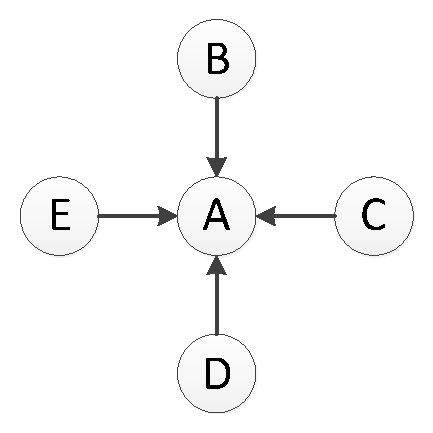
\includegraphics[width=0.25\textwidth]{Diagrams/neighbour-report}}
\caption{Nodes asking for and receiving neighbour data}
\end{figure}

\begin{figure}[H]
  \centering
  \begin{boxedminipage}{\linewidth}
    % 
    \null Process $j$ - \res{neighbourdetect}\\
    %
    \null \textbf{variables}\\
    %
    \null\qq \var{period}: timer init $P_{round}$;\\~\\
    %
    \null\qq \% The history of node\\
    \null\qq \var{previous}: map of address to int init $\emptyset$;\\~\\
    %
    \null\qq \% The current round\\
    \null\qq \var{count}: int init 0;\\~\\
    %
    \null \textbf{constants}\\
    %
    \null\qq \% Round Period\\
    \null\qq \var{$P_{round}$}: time;\\~\\
    %
    \null\qq \% The missed round threshold\\
    \null\qq \var{missed}: int;\\~\\
    %
    \null \textbf{actions}\\
    %
    %
    \null\qq \% Check for changes\\
    \null\qq \emph{round}::~\res{timeout}(\var{period}) $\rightarrow$\\
    \null\qq\qq $\var{previous} \assign \{ (addr, round) \in \var{previous} | count - round \geq missed \}$;\\
    \null\qq\qq \% Tell library caller that a round is finished\\
    \null\qq\qq \res{round-complete}(\res{values}(previous), \var{count});\\
    \null\qq\qq $\var{count} \assign \var{count} + 1$; \\
    \null\qq\qq \res{set}($\mathit{period}$, $P_{round}$); \\~\\
    %
    %
    \null\qq \% Receiving Neighbour Discovery message\\
    \null\qq \emph{neighbour}::~\res{neighbour\_discovery.recv}$\langle source, round\rangle \rightarrow$\\
    \null\qq\qq \% Update the round we last saw this node\\
    \null\qq\qq \res{if} ($source \in \res{keys}(\var{previous})$) \res{then} \\
    \null\qq\qq\qq \res{if} ($round > \var{previous}[\var{source}]$) \res{then} \\
    \null\qq\qq\qq\qq $\var{previous}[\var{source}] \assign \var{round}$; \\
    \null\qq\qq\qq \res{fi}; \\
    \null\qq\qq \res{else} \\
    \null\qq\qq\qq $\var{previous}[\var{source}] \assign \var{round}$; \\
    \null\qq\qq \res{fi}; \\~\\
    %
    %
  \end{boxedminipage}
  \caption{Neighbour Detect Algorithm}
  \label{algo:neighbour-detect}
\end{figure}

For this to be useful we needed a way to get this data back to the sink node. There are many ways to do this, but one of the best is aggregating along a tree because it can combine many messages into a single one and forward that aggregated message instead of lots of smaller messages \cite{?}. The Neighbour Aggregation part uses the Tree Aggregation library that we have developed, the function that is used to aggregate data together is $\cup$ (union), this allows data to be aggregated with other data and allows that data to be updated. The nodes own data is set to be $\res{node-data}$, where $\var{j}$ is the current node's address and $\res{round-data}$ is the set of node addresses provided by the $\res{round-complete}$ callback in \autoref{algo:neighbour-detect}.

\begin{equation}
\res{node-data} = \{\{\var{other}, \var{j}\} | \var{other} \in \res{round-data} \}
\end{equation}


\subsection{Clustering}

\begin{figure}[H]
  \centering
  \begin{boxedminipage}{\linewidth}
    % 
    \null Process $j$ - \res{clustering}\\
    %
    \null \textbf{variables}\\
    %
    \null\qq \% Boolean set to true when a node is elected to be a clusterhead\\
    %
    \null\qq \var{is\_CH}: bool init $False$;\\~\\
    %
    \null\qq \% Bool set to true on receipt of first setup message\\
    %
    \null\qq \var{seen\_setup}: bool init $False$;\\~\\
    %
    \null\qq \% Hop distance to best clusterhead\\
    %
    \null\qq \var{best\_hop}: int;\\~\\
    %
    \null\qq \% Address of best clusterhead\\
    %
    \null\qq \var{our\_CH}: address;\\~\\
    %
    \null\qq \% Newest setup message received\\
    %
    \null\qq \var{msg}: struct;\\~\\
    %
    \null \textbf{constants}\\
    %
    \null\qq \% Detection Time, how long to wait for a better parent after hearing a setup message\\
    \null\qq \var{$T_{detect}$}: time;\\~\\
    %
    \null \textbf{actions}\\
    %
    %
    \null\qq \% Receive new setup message\\
    \null\qq \emph{receive-setup}::~\res{recv}$\langle source, CH, hops\rangle \rightarrow$\\
    \null\qq\qq \% Begin detection timer if this is the first setup message seen\\
    \null\qq\qq \res{if} (¬$seen\_setup$) \res{then} \\
    \null\qq\qq\qq \res{if} ($is\_CH$) \res{then} \\
    \null\qq\qq\qq\qq \res{CH\_detect\_finished}(); \\
    \null\qq\qq\qq \res{else}\\
    \null\qq\qq\qq\qq \res{ctimer\_set}($T_{detect}$,CH\_detect\_finished); \\
    \null\qq\qq \res{fi}; \\
    \null\qq\qq \res{if} ($msg.hop\_count < tmp\_hop\_count$ \&\& ¬$is\_CH$) \res{then} \\
    \null\qq\qq\qq $\var{tmp\_CH} \assign \var{msg.source}$;\\
    \null\qq\qq\qq $\var{tmp\_best\_hop} \assign \var{msg.hops}$;\\
    %
    %
    \null\qq \% End detection period, finalise values\\
    \null\qq \emph{CH\_detect\_finished}::~\res{timeout}(\var{T\_detect}) $\rightarrow$\\
    \null\qq\qq $\var{our\_CH} \assign \var{tmp\_CH}$;\\
    \null\qq\qq $\var{best\_hop} \assign \var{tmp\_best\_hop}$;\\
    \null\qq\qq \% Forward the setup message\\
    \null\qq\qq $\var{newmsg.source} \assign \var{\j}$;\\
    \null\qq\qq $\var{newmsg.CH} \assign \var{is\_CH ? j : our\_CH}$;\\
    \null\qq\qq $\var{newmsg.hops} \assign \var{best\_hop}+1$;\\
    \null\qq\qq \res{stbroadcast\_send\_stubborn}($\var{newmsg}$);\\
    \null\qq\qq \% Inform calling application that setup is complete\\
    \null\qq\qq \res{setup\_complete}();\\
    %
    %
    \null\qq \% Send message placed in buffer by calling application\\
	\null\qq \emph{cluster\_send}::~\res{recv}(\var{newmsg}) $\rightarrow$\\
    \null\qq\qq \res{if} ($is\_CH$) \res{then} \\
    \null\qq\qq\qq \res{runicast\_send}($\var{sink}, \var{newmsg}$);
    \null\qq\qq \res{else}\\    
    \null\qq\qq\qq \res{mesh\_send}($\var{our\_CH}, \var{newmsg}$);
    \null\qq\qq \res{fi}; \\
  \end{boxedminipage}
  \caption{Clustering Algorithm}
\end{figure}

In a wireless network, message collisions are a significant factor in terms of decreasing performance; collisions are more likely in environments featuring a high density of messages. The intuitive solution to this is to reduce the number of messages sent, with minimal compromise in the richness of the data communicated. To this end, we implemented a clustering algorithm. The principle of operation of a clustering algorithm is to establishe a set of clusterheads on network intitialisation. Each of the other nodes in the network allocates itself exactly one clusterhead, through which all traffic to the sink is routed.

In our implementation, the network initialisation phase occurs when an application running on the nodes begins; this application calls the cluster setup routine. The clusterheads are selected to be the set of nodes in the one-hop neighbourhood of the sink. These nodes broadcast their status as a clusterhead to the rest of the network, and the nodes decide with which clusterhead to align themselves based on shortest distance (in hops). Throughout the resmainder of the network's operation, each node passes its messages to the sink through its chosen clusterhead. At this point control is passed back to the application, which can then call the relevant functions to send a message from a node to the sink through that node's clusterhead. As the nature of the setup guarantees that clusterheads will be within one hop of the sink, the messages they pass on from their respective nodes are sent using Contiki's runicast message type. There are no such guarantees for the other nodes, so Contiki's mesh routing is used to allow for arbitrary distance between a node and its clusterhead. This approach to clustering works well when used in small networks, as it achieves its main goal of reducing the number of messages being passed (specifically, the medium will be a lot less congested in the one-hop neighbourhood of the sink). However, this algorithm clearly does not scale well with either geographical distance or number of nodes. In the former case, the majority of nodes will be out of direct transmission range of their clusterhead and will thus have to route messages through several other intermediary nodes; thus increasing the number of messages in the network. Similarly, with large networks a large number of nodes will all need to send messages to clusterheads which form an increasingly small proportion of the network; this is liable to cause bottlenecks and collisions.

\subsection{Hierarchical Clustering}

To counter the given disadvantages of our basic clustering implementation, we developed an additional algorithm which employs the concept of hierarchical clustering. That is, a cluster featuring multiple layers of clusters, each with  clusterhead that has a clusterhead of its own in the next layer. The setup phase of this algorithm also chooses the one-hop neighbourhood of the sink as clusterheads. However, when these clusterheads' setup messages are broadcast through the network, if a node detects that its nearest clusterhead is at least $d$ hops away –- where $d$ is defined as a constant in \verb|contiki.c| –- then that node elects itself as a clusterhead of a new layer, and generates its own setup message to be broadcast. We initially designed two versions of hierarchical clustering; one for arbitrary values of $d$, and one for $d=1$ (where every non-leaf node becomes a clusterhead). However, once the former version was finished we decided to consolidate both versions into one and simply treat $d=1$ as a specific case. To avoid the potential problem of mesh routing creating more messages than the hierarchical clustering saves, in cases of any node being within direct range of its clusterhead, it transmits using runicast. In all other cases, the node uses mesh as before. The hierarchical approach removes the major limitations of our initial clustering implementation, however it still suffers from selecting permanent clusterheads (whereas methods such as LEACH randomise the clusterheads periodically) and thus causing increased power usage for these nodes. Unfortunately, given that clustering is used as a library my some arbitrary application running on the nodes, the implementation of reassigning clusterheads (in any manner of synchronicity) proved infeasible.


\subsection{Predicate Evaluation}

\begin{itemize}
	\item[] Began with single hop predicates
	\begin{itemize}
		\item used Mesh to gather information from surrounding nodes, due to implementation, we could only send one message as a one time
	\end{itemize}	
	\item[] Started work on Multi-hop local based predicates
	\begin{itemize}
		\item used N-Hop Req to send initial message down the chain
		\item We tried using trickle to return the results back to the originating node. However, due to trickles implementation, only one message could be flooded through the network at one time. 
		\item due to collisions, we used ctimers to delay the responses to messages sent back to the originator node.
		\item next step is to re-implement the algorithm, so that nodes send messages directly back along the chain of nodes they recieved the predicated check message from. This way the messages will be more reliably returned to the orignator node. This also allows for multiple messages to be sent this way.
		\item can't really do it via waiting for nodes to respond - difficult to know how long to wait
		\item[] If each node waits (e.g.) 10 seconds, then messages will be lost as they go backwards, as the originating node will have already sent its message back
	\end{itemize}	
\end{itemize}


\subsection{TDMA}

To have a representative algorithm of what may be tested, TDMA (Time Division Multiple Access) was chosen to be implemented and have predicates written for it. The algorithm that was initially implemented was described by \citeauthor{DCATechReport} in \cite[p.~4]{DCATechReport} and is outlined below:

\begin{enumerate}
\item Initially assign every node the smallest numbered channel
\item Every round every node broadcasts a message containing their ID and their currently assigned channel
\item When a message is received the neighbour set is updated and the node that received the message assigns its channel to be the lowest channel not assigned to any neighbour. Two neighbours are not allowed to change their channel in the same round, so a tie breaker is done and the node with the lower ID is allowed to change their channel
\item After choosing a channel the node broadcasts its ID and chosen channel
\item The procedure is repeated until every node cannot choose a smaller channel than its current channel
\end{enumerate}

Interestingly enough when this was first implemented the algorithm only made sure that a node did not have the same channel as any of its one hop neighbours. It did not ensure that the one hop neighbours of any node would have unique channels (as would be required by TDMA to ensure no collisions). This is the kind of bug that running predicates would have assisted identifying.

To make sure that the channel allocation was suitable for TDMA, instead of nodes just sending their own channel assignment to its neighbours. It also included the assignment of the one hop neighbours it knows about in that message. This then allowed nodes to receive information on their two hop neighbourhoods, which they then based their decision on what channel to allocate to themselves from.




\clearpage

% !TeX root = Report.tex
\section{Results}

\subsection{Methodology}

In our simulations we tested networks of various sizes (15, 30 and 48 nodes) aligned in a grid. The nodes were placed such that every node had four neighbours, one to the north, south, east and west, except for nodes in the edge which had three neighbours and the nodes in the corner that had two neighbours. The sink was always placed in the top left corner and was always assigned the address ``1.0''. The predicate checking algorithm was started as soon as the nodes had come online, the nodes then waited for 5 minutes to allow the predicate checking algorithm time to setup and then the TDMA algorithm was started. The simulation was run for 35 minutes overall and then it was terminated. After the predicate checking algorithm had setup the predicate was checked every 2 or 4 minutes depending on the parametrisation. When setting up the Cooja simulator to run the simulations the radio medium was set to be ``UDGM: Distance Loss'', the mote startup delay was set to be 1000ms and a random seed was set to be used on every reload.

To gather metrics on the energy usage of the motes, a Contiki library called rimestats\footnote{\url{http://contiki.sourceforge.net/docs/2.6/a00357\_source.html}} was used. This library is built into the MAC layer and records deep statistics, we simply used the sent and received message counts. In order to calculate how much energy the TDMA algorithm was using we implemented our own sent and received counters that were incremented when a message was sent or received. As the TDMA protocol was implemented with simple broadcasts there should be a one-to-one correspondence between the number of successful broadcasts and the number of transmissions done at the MAC layer, the same is also true for when receiving a message. To calculate the energy cost of the predicate evaluation algorithm, the difference between the total and the TDMA energy usage was taken.

To check that a predicate was successfully evaluated the TDMA algorithm printed any changes in the assigned slot as well as the time the slot was changed. When a predicate was evaluated on a node the time it was evaluated as well as the result was printed. Analysis scripts then evaluated the predicate using the most recent slot value from before or up to when the predicate was evaluated to evaluate the predicate itself. This result was then compared with the actual result of the predicate. The results were compared whether or not the predicate response message reached the sink.

We ran these experiments using two different predicates, one that required 1-hop information and one that required 2-hop information. Both were checking to see if there were slot collisions and were the same two predicate that were mentioned as examples in \autoref{sec:example-predicates}. Below the code and logic for the two predicates is reproduced.

\begin{figure}[H]
\begin{minipage}{.5\linewidth}
\begin{lstlisting}
[all]
function 1 as slot returning int in
    using Neighbours(2) as twohopn in
        @(x : twohopn ~
            slot(x) != slot(this)
        )
\end{lstlisting}
\end{minipage}%
\begin{minipage}{.5\linewidth}
\begin{align*}
&				\forall n \in \text{Nodes} \cdot \\
& \hspace{2em}		\forall n' \in \text{Neighbours}(n, 2) \cdot \\
& \hspace{4em}				\text{slot}(n) \neq \text{slot}(n')
\end{align*}
\end{minipage}

\caption{Check that no two neighbours have the same slot (2-hop information)}
\label{fig:two-hop-slot-pred-lang-results}
\end{figure}

\begin{figure}[H]
\begin{minipage}{.5\linewidth}
\begin{lstlisting}
[all]
function 0 as addr returning int in
function 1 as slot returning int in
    using Neighbours(1) as onehopn in
        @(a : onehopn ~
            @(b : onehopn ~ addr(a) != addr(b)
                => slot(a) != slot(b))
             & slot(a) != slot(this)
        )
\end{lstlisting}
\end{minipage}%
\begin{minipage}{.5\linewidth}
\begin{align*}
&				\forall n \in \text{Nodes} \cdot \\
& \hspace{2em}		\forall n' \in \text{Neighbours}(n, 1) \cup \{n\} \cdot \\
& \hspace{4em}			\forall n'' \in \text{Neighbours}(n, 1) \cup \{n\} \cdot \\
& \hspace{6em}				\text{addr}(n') \not= \text{addr}(n'') \\
& \hspace{8em}					\implies \text{slot}(n') \neq \text{slot}(n'')
\end{align*}
\end{minipage}
\caption{Check that no two neighbours have the same slot (1-hop information)}
\label{fig:one-hop-slot-pred-lang-results}
\end{figure}

\subsection{Analysis}

\begin{figure}[H]
\centering
\subfigure[Rx]{%
	\includegraphics[width=0.44\linewidth]{../Results/Graphs/4.0/1HOP/messagesPE/rx/graph.pdf}
	\label{fig:predeval4.0-rx}
}
\subfigure[Tx]{%
	\includegraphics[width=0.44\linewidth]{../Results/Graphs/4.0/1HOP/messagesPE/tx/graph.pdf}
	\label{fig:predeval4.0-tx}
}

\subfigure[Percentage of  predicates correctly evaluated]{%
	\includegraphics[width=0.44\linewidth]{../Results/Graphs/4.0/1HOP/pcCorrectlyEvaluated/graph.pdf}
	\label{fig:predeval4.0-correct}
}
\subfigure[Percentage of responses received]{%
	\includegraphics[width=0.44\linewidth]{../Results/Graphs/4.0/1HOP/pcResponsesReachedSink/graph.pdf}
	\label{fig:predeval4.0-recv}
}
\caption{Results when predicate period is every 4.0 minutes using a 1-hop predicate}
\label{fig:predeval4.0}
\end{figure}

The first point of note from the data presented in \autoref{fig:predeval4.0} is that in \subref{fig:predeval4.0-recv}, is that both of the global predicate evaluation algorithms (PEGE and PEGP) show a 100\% delivery rate. While this may initially appear very impressive, this simply arises from the facts that these predicates are evaluated at the sink, and that the graph shows the receipt of evaluated predicates sent from the evaluation location to the sink -- as no messages need to be sent, it is vacuously true that no messages will fail to arrive. The two local predicate checking algorithms, however, showed a more predictable trend of successfully delivering fewer responses as the network size increased, though the specific values of these rates are disappointingly low. The values suggest that only nodes in the immediate neighbourhood of the sink are being successful in sending the results of their predicate evaluations. As the network grows in size, the proportion of nodes within this range of the sink decreases, resulting in the trend shown. We believe that this result is due to the way the mesh protocol provided by Contiki works, as it first needs to flood the network with a route discovery message and then waits for a route reply from the target node. However, due to the high amount of traffic it is likely that either or both of these messages are simply being lost. A solution to this would be to have a setup phase, during which every node discovers their respective paths to the sink, before predicate evaluation (or any other main algorithm that is being executed) begins.

Graph \subref{fig:predeval4.0-correct}, showing the rate of correct predicate evaluation, reveals much more useful information: locally-evaluated event-triggered predicates show significantly higher accuracy than each of the other algorithms. Global event-based predicates were shown to have the second-highest accuracy, though this accuracy was only slightly higher than that of the periodic counterpart so it cannot be concluded that an event-based approach is universally better (within the scope of this metric). There may be a connection between PELE having the highest number of received messages (graph \subref{fig:predeval4.0-rx}) and its superior accuracy in evaluation; the premise being that more messages being received could give a node more data to use when evaluating a given predicate, in turn making it more likely to return a correct response. This notion of higher message delivery rates for PELE is somewhat corroborated by the number of transmissions shown in \subref{fig:predeval4.0-tx} -- PELE is responsible for the second lowest number messages sent. However, the cause of PELE alone having a significantly higher success rate in delivering messages is as yet unknown, so more definitive information on this front would require further scrutiny using testing methods that may well prove infeasible in a resource-constrained system.

It is also good to note that as the network size increases the correctness of predicate evaluation remains effectively constant, with only small fluctuations. From this we can say that the predicate evaluation libraries are highly scalable with respect to the size of the network and the accurate evaluation of the predicate. However, as has been mentioned before they scale poorly with respect to the number of responses the reach the sink.

As messages sent and received use the most energy in a WSN system \cite{Shnayder04} we will use message transmit and receive statistics to evaluate the energy usage of the algorithms. In graphs \subref{fig:predeval4.0-rx} and  \subref{fig:predeval4.0-tx}), local periodic predicate evaluation is the most conservative, however it also shows the lowest accuracy for its evaluations so these results show little in the way of benefits to using this algorithm. By contrast, the most accurate algorithm, PELE, has a higher (yet still moderate) level of energy consumption. An important observation is that the energy demands of global predicate evaluation -- both of which showed middling accuracy -- increase faster than those of local evaluation as network size increases. This is because global evaluation requires data from the entire network, and the operating of the mesh routing protocol means that nodes lying further from the sink will have to have their messages forwarded by a greater number of intermediate nodes, giving exponential growth in the number of messages sent. The local evaluation algorithms show a more linear trend as the size of a node's 1- or 2-hop neighbourhood may not increase due to the presence of more nodes in the network -- all that is guaranteed is that there will be more such neighbourhoods in which to evaluate predicates.

\begin{figure}[H]
\centering
\subfigure[Rx]{%
	\includegraphics[width=0.44\linewidth]{../Results/Graphs/2.0/1HOP/messagesPE/rx/graph.pdf}
	\label{fig:predeval2.0-rx}
}
\subfigure[Tx]{%
	\includegraphics[width=0.44\linewidth]{../Results/Graphs/2.0/1HOP/messagesPE/tx/graph.pdf}
	\label{fig:predeval2.0-tx}
}

\subfigure[Percentage of predicates correctly evaluated]{%
	\includegraphics[width=0.44\linewidth]{../Results/Graphs/2.0/1HOP/pcCorrectlyEvaluated/graph.pdf}
	\label{fig:predeval2.0-correct}
}
\subfigure[Percentage of responses received]{%
	\includegraphics[width=0.44\linewidth]{../Results/Graphs/2.0/1HOP/pcResponsesReachedSink/graph.pdf}
	\label{fig:predeval2.0-recv}
}
\caption{Results when predicate period is every 2.0 minutes using a 1-hop predicate}
\label{fig:predeval2.0}
\end{figure}

At first glance of figure \autoref{fig:predeval2.0} the results seem to mirror those of figure \autoref{fig:predeval4.0}, however there is a key difference, in that the performance of the global periodic-based implementation had a lower success rate, when the predicate period is 2.0 minutes. This is likely due to the fact that messages are sent more often, and are therefore causing more collisions, losing messages, ultimately resulting in a lower success rate. 

The graphs also show that there were a larger number of messages both sent and received in these tests (figures \autoref{fig:predeval2.0-rx} and \autoref{fig:predeval2.0-tx}), although this can be attributed to the fact the predicate period is more often, requiring more messages to be passed around the network. Comparing the two sets of data we can see there were similar performance levels, regardless of the predicate period length. It can also be suggested that increasing the predicate period would increase the evaluation success rate, as there would be less collisions for the network to deal with. Of course, based on the above reasoning, increasing the period would also decrease the number of messages sent by the periodic implementations and would thus extend battery life.

\begin{figure}[H]
\centering
\subfigure[Rx]{%
	\includegraphics[width=0.44\linewidth]{../Results/Graphs/4.0/2HOP/messagesPE/rx/graph.pdf}
	\label{fig:predeval2hop-rx}
}
\subfigure[Tx]{%
	\includegraphics[width=0.44\linewidth]{../Results/Graphs/4.0/2HOP/messagesPE/tx/graph.pdf}
	\label{fig:predeval2hop-tx}
}

\subfigure[Percentage of predicates correctly evaluated]{%
	\includegraphics[width=0.44\linewidth]{../Results/Graphs/4.0/2HOP/pcCorrectlyEvaluated/graph.pdf}
	\label{fig:predeval2hop-correct}
}
\subfigure[Percentage of responses received]{%
	\includegraphics[width=0.44\linewidth]{../Results/Graphs/4.0/2HOP/pcResponsesReachedSink/graph.pdf}
	\label{fig:predeval2hop-recv}
}
\caption{Results when predicate period is every 4.0 minutes using a 2-hop predicate}
\label{fig:predeval-2hop-4.0}
\label{fig:predeval2hop}
\end{figure}

The previous two sets of results in \autoref{fig:predeval4.0} and \autoref{fig:predeval2.0} were for the 1-hop variant of the TDMA slot collision predicate. In \autoref{fig:predeval-2hop-4.0} results for the alternative 2-hop predicate are shown. There are a number of patterns that differ and some that remain the same.

To begin with we observe the same behaviour with respect to the delivery ratio of failure response messages. Predicates that are evaluated at the root node of the tree continue to have a 100\% delivery rate, while nodes evaluating in-network continue to have poor delivery rates that decrease in larger networks. The issue here is the same as the problem encountered with the 1-hop predicate results, so the same solution proposed would apply here.

Next, we have very different patterns of number of messages sent. We find that PELE requires the largest amount of energy to operate and PELP requires the least, with both growing linearly with respect to network size, whereas the global predicate evaluators use energy between these two levels and this energy increases faster than linearly. The difference here is that it is no longer the case that global evaluators require the most number of message to be sent. In fact the global evaluators use almost the same number of messages when comparing the 2-hop predicate results to the 1-hop predicate results. This is because the structure of sending messages to a node for predicate evaluation is the same in both 1-hop and 2-hop predicate evaluation, it is via an aggregation tree. The local in-network predicates are where large increases in messages sent occur. These increases are down to the fact that the neighbourhood of information that needs to be disseminated has increased from 1-hop to 2-hops. We see that this affects PELE more than it does PELP, for example for size 15 networks both local predicate evaluators transmit about 1000 message when evaluating the 1-hop predicate, whereas when evaluating the 2-hop predicate PELP sends about 1500 messages and PELE sends 2500 messages. So it when increasing the size of data that needs to be requested our event-based predicate evaluator will send more messages.

There is also a very interesting difference with respect to the correctness of predicate evaluation. When evaluating the 1-hop predicate the local in-network event-based evaluator performed best. However, for the 2-hop the local periodic evaluator performed best, we would expect that usually this would have been caused by the increase in message transmissions leading to a busier network with more collisions and message lost. Except that as the network size increases the number of messages transmitted increases, but the percentage of predicates that were correctly evaluated remains the same, so it would initially appear that collisions do not factor in. On the other hand, because these predicates are evaluated in-network they are by definition local, so increases in messages transmitted across the whole network may not paint an accurate picture. What we believe to be the case is that, compared to the 1-hop predicate, the 2-hop predicate has more local traffic and thus more local collisions which lead to event-based in-network evaluators to perform badly as lots of redundant data is transmitted. However, with in-network periodic evaluators data is only transmitted when it is asked for. So while event-based data sending may have helped for 1-hop predicates with respect to the greater number of transmissions, due to the increased number of hops data needs to travel to evaluate 2-hop predicate sending data when it changes actually leads to more local collisions leading to less current data reaching nodes, causing event-based evaluators to perform worse for 2-hop predicates than 1-hop predicates.

Another point is that for 2-hop evaluation the percentage of predicates correctly evaluated is generally lower than when evaluating 1-hop predicates. This is likely caused by the fact that more data is required, so there is a greater chance for more of it to be out-of-date by the time it reaches the evaluating node. There is also a greater chance for not all the data to reach the node evaluating the predicate (as there is simply more data being transmitted). Either of these two issues could have lead to the overall decrease in accuracy of evaluating the predicate.


\clearpage

% !TeX root = Report.tex
\section{Practical Experience}

\subsection{Sensor Data Conversion}
Sensors didn't provide data in human understandable formats. Instead they were provided in a raw format that were dependant on several hardware properties of the sensors (such as voltage levels and the number of bits of data a sensor can report). So we  had to convert from raw sensor data to expected results using equations found in \cite{sensiriondatasheet}.

\subsection{Uploading to the motes}
Command used
\begin{listing}
\begin{minted}[fontsize=\small]{bash}
sudo make example-unicast.upload DEFINES=HELLOWORLD,NODE_ID=1 MOTES=/dev/ttyUSB0
\end{minted}
\end{listing}
Adding .upload to the end of the project name, will start the upload to the motes. The MOTES variable is used to locate the USB port for the mote.

The NODE\_ID is used to set the rime address on the nodes. Provided the following macro is inserted into the code. This is important to do because otherwise the MAC address of the node will not be set. Even if the rime address of the node is set, the lack of a MAC address will cause message sent with unicast primitives to fail to arrive, as the address is not correctly set.

\begin{listing} 
\begin{minted}[fontsize=\small]{c}
#ifdef NODE_ID
node_id_burn(NODE_ID);
#endif
\end{minted}
\end{listing}


\subsection{Power Levels}
Using the low power levels (3 or lower) resulted in very unreliable transmission rates/distances. We believe that this was caused by the environment that we were testing in (DCS building), which we expect the traffic on the 2.4GHz frequency to be very busy due to the number of phones and wireless devices in the department.

\subsection{Transmission Ranges}
When developing our mote applications in the simulator there is a very useful feature that allows one to see what the transmission radius of a selected node is. This help developers to work out what the expected behaviour of a piece of software should be. When developing in real-world scenarios, we found that we were never quite sure if our software was simply not working in a real-world environment or if the motes were placed too close to each other or too far.

\subsection{Communication Between Mote and Computer}
To be able to send and receive information between an application running on a mote and an application running on the computer the mote is connected to we needed to use several applications to assist in the data transfer. The easiest flow of data was from the mote to the computer as Contiki supports writing to \verb|stdout| which can then be read using a tool called \verb|serialdump|. Unfortunately Contiki doesn't support writing to \verb|stdout| so we had to develop and alternative method to read data sent from a computer. Also when sending data from the computer application to the mote application we couldn't simply open a filestream in Java and write to that (and expected Contiki to receive it), so we also had to come up with a custom way to do this.

\subsubsection{Receiving Data from Nodes}

\url{http://ai.vub.ac.be/Robotics/wiki/index.php/Compiling,_uploading_and_interacting_with_Contiki:_Hello_World}

\subsubsection{Sending Data to Nodes}

\url{https://github.com/contiki-os/contiki/wiki/Input-and-output#wiki-Serial_Communication}


\subsubsection{Simulating with Cooja}

Use the \verb|serial_socket| plugin to create a serial server or client for a given node. Connect to these via sockets and communicate that way.

\subsection{Developing with Small Message IDs}

When using small message identifiers, after sending enough messages the variable used to hold the identifier will overflow. This make testing if a message has come after another message slightly difficult.

\subsection{Setting up serial2pty Cooja Plugin}

\begin{listing}[H]
\begin{minted}[fontsize=\small]{bash}
cd ~/contiki/tools/cooja/apps
git clone git://i4git.informatik.uni-erlangen.de/contiki_projects.git -b serial2pty serial2pty
cd serial2pty
ant jar
\end{minted}
\end{listing}

Now you can load this plugin in Cooja by going to \verb|Settings| \verb|->| \verb|Cooja Extensions| and selecting serial2pty. Once it has been selected click \verb|Apply for session| and \verb|Save| and the plugin will now be enabled. To run it simply \verb|Tools| \verb|->| \verb| Serial 2 Pty| \verb|->| and select the node you want to connect. You will be told what device you can connect to, to receive the serial output from.

Initially we found that this tool would not build, so a patch was created to fix those issues, sent to the developer and it was integrated into the repository.

\subsection{Cooja Memory Usage  and Options}

We found that Cooja's default settings when run using \verb|ant run| were suitable for smaller networks. However when running more memory intensive applications on the simulator of the hardware in Cooja or when running larger networks, Cooja itself can run out of memory. The simple solution is to simply run Cooja using \verb|ant run_bigmem| which supplies a flag limiting the maximum about of memory to 1536MB instead of 512MB when running normally \cite{?}.

As Cooja is written in Java \cite{?} it means that all of Java's configuration flags are also up for modification. This however, means that the \verb|ant| build script at \verb|~/contiki/tools/cooja/build.xml| will need to be modified to include the flags that need to be passed to Java. We modified the build script to add the following arguments (\verb|-XX:+OptimizeStringConcat| \verb|-XX:UseSSE=3| \verb|-XX:+UseFastAccessorMethods| \verb|-XX:+UseLargePages|) but did not see much improvement of performance.

Finally, there is one other useful mode, and that is the ability to run Cooja without a GUI. This is done by changing the run command to \verb|ant run_nogui|. Running in this mode is very useful when running many simulations to obtain results from them as fast as possible.


\subsection{Static variables}

When developing libraries make sure you use static variables vary carefully. For example we found that commonly we would make callback timers static and then use that object. When the code using that timer will only be called from one place it is okay. However, when you have multiple calls to that timer (imagine broadcasting on different channels) this can cause race conditions as the memory for that timer is being shared. What should be done is the timer object should be placed in a struct and that struct should be passed to the relevant functions that need to access the timer. For each time you wish to use the library a pointer to a different struct should be passed to those functions.

However, there are times that declaring a variable as static is very important. One of these cases is when you have a process that it waiting on some event, if you want a variable to maintain the same value after the event has been waited on, then that variable needs to be static. In \autoref{lst:contiki-process-static-variables} the \verb|printf| statmenet prints out a static and non-static variable. The static counter will increase and be reliably printed out. However, when the variable \verb|x| is printed, the value it contains at that point could be anything. This is due to the way that Contiki's process are actually proto-threads, so share a stack with other proto-threads, if another process were to be scheduled at this point it could potentially modify the stack. This would lead to stack variables such as \verb|x| potentially being changed. On the other hand, if there are no points in the program where the process may yield to other threads, then variables can be non-static. For example \verb|y|'s value would be printed correctly every time.

\begin{listing}[H]
\begin{minted}[fontsize=\small]{c}
PROCESS_THREAD(proc, ev, data)
{
	static struct etimer et;
	static unsigned int counter = 0;

	PROCESS_BEGIN();

	while (true)
	{
		unsigned int x = 1234;

		etimer_set(&et, 10 * CLOCK_SECOND);
		PROCESS_WAIT_EVENT_UNTIL(etimer_expired(&et));

		unsigned int y = 2;

		printf("%u %u %u\n", counter, x, y);

		++counter;
	}

	PROCESS_END();
}
\end{minted}
\caption{Contiki process static variables}
\label{lst:contiki-process-static-variables}
\end{listing}

\subsection{Firmware Size}







\clearpage

% !TeX root = Report.tex
\section{Project Management}

\subsection{Methodology}

The requirements of the project was not fully understood at the beginning and we were unsure of the efficiency of our algorithms so we decided to go for a prototyping approach as part of an evolutionary process model. This allows us to start with a set of core product and system requirements (i.e. the operating system) and then incorporate other extensions as the requirements are better understood. We also had frequent meetings with our supervisor to discuss the best ways to implement our system and any additional components. Where a new idea is defined, a prototype is modelled and constructed and is re-evaluated by our supervisor, who provides feedback which is used to further refine the requirements. This process is repeated until the supervisor is satisfied with the function of the system, while at the same time enabling us to better understand what needs to be done.

\subsubsection*{Term 1}

We spent the first few weeks researching on the different aspects of wireless sensor networks as well as the appropriate tools and platform to develop our system. Some concepts such as broadcasting consists of numerous methods where each are tailored to work best in different systems and working environments. Since this is beyond our practical knowledge, we had to implement most of the methods and tested it on the system to determine the most efficient one. With this proceeding, it was hard to define the overall scope of our project since there were many factors that had to be considered. Nevertheless, we produced a list of all the possible algorithms and protocols to implement and ranked them according to its relevance. We followed a 'dive-in' procedure by implementing the most relevant components first and updated the list by removing or adding algorithms.

%Can state here what was said in the feedback form. nahh

\subsubsection*{Term 2}

At this stage, most of the algorithms and protocols were implemented independently and treated as individual components to the core system. We decided to do it this way because of the benefits of modularity where the principles of "Separation of Concerns" allows for a more manageable set of modules. The composition of these components such as predicate checking and neighbour data retrieval was done during the entire winter vacation and the beginning of the second term.
%We can mention here a small list of the algorithms that needed to be integrated together

In the second term, we continued following the evolutionary process model but at a more relaxed approach which focuses on finishing the system components and preparing the gathering of results. Since the project scope was clear and we had a more directed goal,less meetings with the supervisor was needed, but we still required him to evaluate our work and provide feedback. Ensuring that the development and debugging phase to complete in time required the effective scheduling of tasks and prioritising work force to the critical ones. By the third quarter of the term, progress had fallen to a halt due the high number of coursework deadlines and this meant that team members where preoccupied with other duties. To address the issue, a meeting was held prior to the halt where we discussed our recovery plan and actions to take once members was free. This allowed team members to continue working where they left off and avoid any delays.

\subsection{Role Allocation}

We decided to allocate roles in the second week after we had the first week to perform research into the problem and find out what has been done. The following were how we assigned roles, although we intend for these to be flexible:

\begin{table}[H]
\centering
	\begin{tabular}{| c | c |}
		\hline
		Name & Role\\
		\hline
		Matthew Bradbury & Group Leader\\
		Daniel Robertson & Project Manager\\
		Amit Shah & Technical Leader\\
		Ivan Leong & Developer and Tester\\
		Joe Yarnall & Developer and Tester\\
		Tim Law & Developer and Researcher\\
		\hline
	\end{tabular}
\end{table}

Whilst the entire team was responsible for system design and development, it was critical to have a group leader and other leading roles to facilitate and provide resources to the team. Their individual responsibilities is as follows:

\begin{itemize}
	\item[] {\bf Matthew Bradbury} - Group Leader
	
	His main task is to lead the entire project and have a clear understanding of the components that is to be implemented. He is responsible for allocating tasks to its team members and providing direction for meeting the project objectives.He also possesses strong communication skills with his team members as well as being able to explain the concepts to the supervisor concisely.Ensures that everyone is performing their roles accordingly and providing motivation when the project is slowing down.	

	\item[] {\bf Daniel Robertson} - Project Manager
	
	He supports the group leader by facilitating the management of the project and ensuring that the overall work is done on schedule. He arranges weekly meetings and provides a summary report prior to each meeting and records all discussions.
	
	\item[] {\bf Amit Shah} - Technical Leader
	
	Responsible for overseeing the work done by other members and ensures that all code written by the team meets the technical specification and design requirements of the project.	
	
\end{itemize}

\subsection{Project Planning}

Our initial planning was done in the first few group meetings and most of the plan details was explained in the project specification. As we progressed through the project development, we encountered many changes from the initial plan as well as changes in task schedule. This section presents the final overall plan of the project including the revised time schedule of development activities, resources used and issues encountered.

\subsubsection{Work Breakdown Structure}

The figure below shows the work breakdown structure as designed for the project specification.

\begin{figure}[H]
\centering
\includegraphics[width=\linewidth]{Images/pm-wbs.pdf}
\caption{Work Breakdown structure}
\label{fig:Work Breakdown Structure}
\end{figure}

\subsubsection{Deliverables}

Our project consists of 5 deliverables which includes one individual report. It was very important that these milestones were met because it allows us to monitor our progress and prove that we were working in the direction of the stated goals and requirements of the project.

\begin{enumerate}
	\item Specification \emph{(Due Week 4 - Term 1)}
	
	This was the first deliverable of the project. At the time, we were still undergoing research on the different components of the system and the project scope was not clearly defined. Nevertheless, we highlighted in the specification the main goals of our project and the different algorithms that we wished to implement. We also included a schedule of all the planned activities for the remainder of the project and an approximate time taken to complete them.
	
    \item Progress Poster Presentation \emph{(Due Week 10 - Term 1)}
    
	By the end of the first term, the scope of the project had reached a more defined level as we had decided what is to be implemented and what has been disregarded from the provisional list of algorithms. This was demonstrated in our first delivery - the poster presentation, where we had to chance to explain our project at a high level to our supervisors and other professors.
    
    \item Final Group Report \emph{(Due Week 1 - Term 3)}
    
	Although the report is due in term three we started adding content since the first term. This included the introduction, literature review, a list of algorithms and protocols to be implemented and a brief description of their functions. In the beginning of the second term, much of the algorithms were described in the report and it was only towards the end of the term that the report was being updated on a full scale. Each member was assign a specific section to work on but with the flexibility to update other sections if it was related to them.
	
    \item Individual Report \emph{(Due Week 1 - Term 3)}
    
	Every team member needs to write a 3000 words report to reflect on their performance and contribution towards the project as an individual.
    
    \item Final Project Presentation \emph{(Due Week 3 - Term 3)}
    
    Demonstrate our final project to a judge of panels and supervisor.
 
\end{enumerate}

\subsubsection{Schedule}

Throughout the term, every member was assigned specific tasks and was given a time frame to complete them. The table below shows the time schedule allocated to each members.

\begin{table}[H]
	\centering
	\begin{tabular}{| l | l | l | l | l | l | l |}
	\hline
	Task Description & \multicolumn{6}{l|}{Time Allocated (Weeks)}\\
	~ & Amit & Dan & Ivan & Joe & Matt & Tim \\
	\hline
	\hline
	\multicolumn{7}{|l|}{\textbf{Term 1} - Developing for application predicate checking} \\
	\hline


	Research around the Problem & 2 & 2 & 2 & 2 & 2 & 2\\
	Writing Specification & 1 & 1 & 1 & 1 & 1 & 1\\
	H-SEND Implementation & 3.5 & ~ & ~ & 3.5 & ~ & ~\\
	``Send to Base'' Implementation & ~ & ~ & ~ & ~ & 2 & 1.5\\
	Clustering Implementation & ~ & 3.5 & 2 & ~ & ~ & ~\\
	Aggregation Tree Implementation & ~ & ~ & ~ & ~ & 1.5 & ~\\
	Develop Visualisation Tool & ~ & ~ & 1.5 & ~ & ~ & 2\\
	Develop Predicate Language Runtime & ~ & ~ & ~ & ~ & ~ & 2\\
	Testing and Adapting to Physical Nodes & 2 & 2 & 2 & 2 & 2 & 2\\
	Message Logging & ~ & ~ & ~ & 1 & ~ & ~\\
	Poster Creation and Presentation preparation & 1.5 & 1.5 & 1.5 & 1.5 & 1.5 & 1.5\\

	\hline
	\hline
	\multicolumn{7}{|l|}{\textbf{Term 2} - Developing for network predicate checking and where the predicate is checked} \\
	\hline
	
	Additional Research & 1 & 1 & 1 & 1 & 1 & 1\\
	Improving Dynamic Predicate Specification & 2 & 2 & ~ & ~ & 2 & 2\\
	Develop Visualisation Tool & 2 & ~ & 2 & 2 & ~ & 2\\
	Modify Algorithms to Selectively Evaluate Predicates & ~ & 2 & 2 & 2 & 2 & ~\\
	Performance Testing & 1.5 & 1.5 & 1.5 & 1.5 & 1.5 & 1.5\\
	Testing and Adapting to Physical Nodes & 1.5 & 1.5 & 1.5 & 1.5 & 1.5 & 1.5\\
	Report Writing & 2 & 2 & 2 & 2 & 2 & 2\\
	\hline
	
	\end{tabular}
\end{table}

\subsubsection{Gantt Chart}

The project plan was adhered to as much as possible and was closely monitored as shown in the Gantt chart below. The Gantt chart was edited several times and accounted for revisions made whenever there was a change in task or time schedule. The colours of the bars are as follows:

\begin{itemize}
	\item[] Green: Research and learning
	\item[] Orange: Design
	\item[] Blue: Implementation
	\item[] Yellow: Specification and report preparation
	\item[] Red: Testing
\end{itemize}

\begin{figure}[H]
\centering
\includegraphics[height=.99\textheight]{Images/pm-gantt.pdf}
\caption{Gantt Chart}
\label{fig:Gantt Chart of project}
\end{figure}

\subsection{Resources}
% Can explain more on the software we used to share resources, communicate and discuss ideas.

\subsubsection{Working Concurrently}

We signed up for a Git repository on BitBucket \cite{bitbucket} where we plan to commit all the work we produce. We initially had an issue that free private repositories hosted on BitBucket have a maximum of 5 participants, whereas we had 6 group members. Fortunately when new users sign up to the services from an invite, the person that sends the invite gets additional capacity. This meant that the person who created the repository ended up with enough capacity for all members to access the account. The use of BitBucket also gives the advantage of branching and merging codes from different users without needing to replicate any files and worry about redundancy. 

\subsubsection{Communication}

When group members are working offline, the main source of communication is via the popular social networking platform - Facebook. We created a group for our team where members could post any messages regarding the project such as issues in code development, assignment of tasks to team members and reminders of any project activities (e.g. weekly meetings).

\subsubsection{Development tools}

The following table summaries all the software and hardware used to develop the wireless sensor network application. 


%To add more items increment multirow

\begin{table}[H]
\centering
\begin{tabular}{| l | p{2.5cm} | p{4.5cm} | p{4.25cm} |}
	\hline
	~ & Name & Description & Constraints/Issues\\
	\hline

	\multirow{6}{*}{Software} & Contiki & Operating System for WSNs & ~
	
	\\ \cline{2-4}

	& Cooja & Contiki Simulator & ~
	
	\\ \cline{2-4}

	& Bash and Python & Scripting numerous tasks & Some dependencies had to be manually installed\\ 
	\cline{2-4}

	& Make & To compile the C source code for the project & ~\\ 
	\cline{2-4}

	& MSP-GCC & The custom compiler used & Did not come installed on DCS computers, needed to compile ourselves\\ 
	\cline{2-4}

	& Netbeans and Java & To develop the GUI & ~\\ 
	\hline

	\multirow{2}{*}{Hardware} & Sensor nodes & See \autoref{sec:dev-spec} & Provided by department, needed to share with PhD student who also required them\\ 
	\cline{2-4}

	& USB Hub and USB cables & To work with multiple sensor nodes at once & Hub required purchasing, cables were borrowed from DCS\\
	\cline{2-4}
	
	\hline

\end{tabular}
\end{table}


\subsection{Risk Analysis}
%Potentially the issues below can form part of risk
It is almost certain that every project contains risks which could impact its progress and success if not well managed. Risk management involves two basic steps, 1) to identify the different possible risks that may occur in the project and its likelihood of occurrence and 2) state the actions to mitigate the effects of any threats.

\begin{center}
	\begin{longtable}{| p{4cm} | l | l | p{7cm} |}
	\hline
	Risk & Likelihood & Severity & Mitigation\\
	\hline	
	
	Hardware and Software failure
	\begin{itemize}
		\item Report and research
		\item Software code
	\end{itemize}
	 & 2 & 9 & To prevent the risk of data lost, we used a Bitbucket repository to save and store all our documents and program coding online. This also allows the concurrent development of our project and ensuring that all team members are up to date.
	 
	\\ \hline
	
	Team member illness and absence
	& 5 & 4 & There would be circumstances where team members would be unavailable to work on the project for a short period of time. To ensure that work is progressive, necessary measures were taken. For example an absent member can temporary delegate his current task to a different member.
	
	\\ \hline
		
	Meeting deadlines and schedules
	& 5 & 7 & It was important that every milestone of the project was met so that no marks were penalised. The progress of the project was monitored and we had weekly meetings to ensure that everyone was on track of their given tasks.
	
	\\ \hline
	
	Obtaining desired results when deploying code (tested on simulated environment) on physical devices
	& 5 & 5 & Most of the code that was developed in the beginning was tested with the Cooja simulator. It would be unlikely to obtain similar results when deployed on the actual hardware due to a wide range of environmental factors such as interference and power distribution. An option is to gather data from simulated environment rather than physical devices.
	
		\\ \hline
		
	Defining the scope of our project
	& 5 & 5 & There are many issues and research problems that revolve around the topic of wireless sensor networks. It is important to define the scope of the project to prevent scope creep and necessary expansion of the project.

Need to keep track of all new ideas proposed by the supervisor and raise any change requests to the project.

		\\ \hline
		
	Damage of the sensor nodes
	& 3 & 5 & Each of the sensor nodes cost 80 Euros. The sensors must be handled with care to prevent any cost of damage. Assign a group member the responsibility to store the sensors after use and keep track of who is using them.
	
		\\ \hline
		
	Components of the project that could not be implemented with current tools.
	& 4 & 4 & Research on alternative methods or implement custom tools.
	\\ \hline		
		
	\end{longtable}

\end{center}

\subsection{Work Overview}

This section highlights the different tasks that was undertaken by each group member for every week of term 1 and term 2. At every weekly meetings, the project leader would discuss the progress of the tasks that was assigned in the previous week and any new tasks for the current week would be recorded as shown in the table below.
%perhaps number the table below 

\subsubsection*{Term 1}

\begin{center}
	\begin{longtable}{| l | p{9cm} | p{3.5cm} |}
	\hline
	Week & Activities & Task Allocation\\
	\hline
	1 & \begin{enumerate}
			\item Meet up with Supervisor and discuss project direction
			\item Research on related work and what we can develop, before settling on main aims
			\item Investigate two OS and their corresponding simulators: TinyOS with TOSSIM and Contiki with Cooja
		\end{enumerate} &
	\begin{enumerate}
		\item[] Amit: All
		\item[] Dan: All
		\item[] Ivan: All
		\item[] Joe: All
		\item[] Matt: All
		\item[] Tim: All
	\end{enumerate}
	\\ \hline

	2 & \begin{enumerate}
			\item Research if Cooja can be extended through the use of plug-ins (with the aim of extending it to replay traffic logs)
			\item Research Clustering algorithms and find implementations
			\item Develop a temperature dissemination application to learn Contiki and Cooja
			\item Research TinyOS and TinyDB and see if they could be applied to predicate checking
			\item Investigate performance of different MAC protocols
			\item Investigate the feasibility of live monitoring of the network
			\item Investigate QoS and how it may be applied to real life WSN deployments
			\item Produce a literature review on chosen topic
		\end{enumerate} &
	\begin{enumerate}
		\item[] Amit: 1, 7, 8
		\item[] Dan: 5, 8
		\item[] Ivan: 6, 8
		\item[] Joe: 4, 8
		\item[] Matt: 3, 8
		\item[] Tim: 2, 8
	\end{enumerate}
	\\ \hline
	
	3 & \begin{enumerate}
			\item Research DICAS
			\item Research Send to Base
			\item Research Daicon
			\item Research DIDUCE
			\item Research H-SEND
			\item Research Sympathy
			\item Write Specification
		\end{enumerate} &
	\begin{enumerate}
		\item[] Amit: 2, 7
		\item[] Dan: 4, 7
		\item[] Ivan: 3, 7
		\item[] Joe: 1, 7
		\item[] Matt: 6, 7
		\item[] Tim: 5, 7
	\end{enumerate}
	\\ \hline
	
	
	4 & \begin{enumerate}
			\item Finish Specification
			\item Work out how to get MSP430-GCC and the Cooja working on Joshua
			\item Begin developing aggregation tree example
		\end{enumerate} &
	\begin{enumerate}
		\item[] Amit: 1, 2
		\item[] Dan: 1
		\item[] Ivan: 1
		\item[] Joe: 1
		\item[] Matt: 1, 3
		\item[] Tim: 1
	\end{enumerate}
	\\ \hline
	
	
	5 & \begin{enumerate}
			\item Get used to developing in C and learn how to use the Contiki libraries
			\item Finish developing aggregation tree
			\item Start implementing clustering algorithms
			\item Start implementing H-SEND
		\end{enumerate} &
	\begin{enumerate}
		\item[] Amit: 1, 4
		\item[] Dan: 1, 3
		\item[] Ivan: 1, 3
		\item[] Joe: 1, 4
		\item[] Matt: 1, 2
		\item[] Tim: 1
	\end{enumerate}
	\\ \hline
	
	
	6 & \begin{enumerate}
			\item Start Implementing GUI
			\item Implementing clustering algorithms (Regular and Hierarchical)
			\item Implement H-SEND
			\item Implement a local predicate checker and reporter
		\end{enumerate} &
	\begin{enumerate}
		\item[] Amit: 3
		\item[] Dan: 2
		\item[] Ivan: 2
		\item[] Joe: 3
		\item[] Matt: 4, 2
		\item[] Tim: 1
	\end{enumerate}
	\\ \hline
	
	7 & \begin{enumerate}
			\item Library-ify Cluster implementations
			\item Implement LEACH  using existing implementations as a base
			\item Work out how to interface the GUI and the base station
			\item Continue developing GUI
			\item Get in contact with Sain Saginbekov and sort out when we can use sensor nodes
			\item Contact Victor Sanchez and inform him when we are using sensor nodes
			\item Implement multi-hop predicate checking
			\item Slim down eLua enough for us to run it on the sensor nodes, to allow for dynamic predicate specification
			\item Research and start implementing network traffic logging and reporting
		\end{enumerate} &
	\begin{enumerate}
		\item[] Amit: 7
		\item[] Dan: 1, 2
		\item[] Ivan: 9
		\item[] Joe: 5, 6, 7
		\item[] Matt: 8
		\item[] Tim: 3, 4
	\end{enumerate}
	\\ \hline
	
	8 & \begin{enumerate}
			\item Start work on poster with the aim of finishing it by the end of week 9
			\item Detect and report neighbours for display in the visualisation tool, aim to be able to work in mobile networks, with gained and lost neighbours
			\item Log network data and report it to the network (for visualisation tool to replay traffic)
			\item Finish predicate language parser and code generation
			\item Tidy up n-hop HSEND
			\item Integrate n-hop HSEND with predicate language virtual machine
			\item Experiment with interference affecting node communications
		\end{enumerate} &
	\begin{enumerate}
		\item[] Amit: 1, 5, 6
		\item[] Dan: 1, 3, (~7)
		\item[] Ivan: 1, 2, (~7)
		\item[] Joe: 1, 2, (~7)
		\item[] Matt: 1, 4, 6
		\item[] Tim: 1, 4
	\end{enumerate}
	\\ \hline

	9 & \begin{enumerate}
			\item Create poster for presentation
		\end{enumerate} &
	\begin{enumerate}
		\item[] Amit: 1
		\item[] Dan: 1
		\item[] Ivan: 1
		\item[] Joe: 1
		\item[] Matt: 1
		\item[] Tim: 1
	\end{enumerate}
	\\ \hline

	10+ & \begin{enumerate}
			\item Code generation for predicate language
			\item Network visualisation (node neighbours)
			\item GUI to Node interface
			\item Message logging
			\item Neighbour Reporting
			\item Turn existing code into libraries
			\item Make existing code handle generic data
			\item Integrate predicate evaluating VM and neighbour data retrieval
			\item Write up notes on work done this term
		\end{enumerate} &
	\begin{enumerate}
		\item[] Amit: 6, 7, 8, 9
		\item[] Dan: 4, 5, 9
		\item[] Ivan: 3, 5, 9
		\item[] Joe: 6, 7, 8, 9
		\item[] Matt: 6, 7, 8, 9
		\item[] Tim: 1, 2, 9
	\end{enumerate}
	\\ \hline
	
	\end{longtable}
\end{center}

\subsubsection*{Term 2}

\begin{center}
	\begin{longtable}{| l | p{7.5cm} | p{5cm} |}
	\hline
	Week & Activities & Task Allocation\\
	\hline
	1 - 2 & \begin{enumerate}
		\item Continue network visualisation
		\item Interface Base station node with desktop application
		\item Develop neighbour detection and reporting to sink
		\item Integrate predicate evaluating, predicate VM and neighbour data retrieval
		\item Finish parser and compiler of predicate language
		\end{enumerate} &
	\begin{enumerate}
		\item[] Amit: 4
		\item[] Dan: 3
		\item[] Ivan: 2
		\item[] Joe: 4
		\item[] Matt: 4, 5
		\item[] Tim: 1
	\end{enumerate}
	\\ \hline

	3 & \begin{enumerate}
		\item Continue network visualisation
		\item Interface Base station node with desktop application
		\item Develop type checker for predicate language
		\item Find bug that is causing unicast communications to fail
		\item Develop a way to handle packets larger than the maximum broadcast size
		\end{enumerate} &
	\begin{enumerate}
		\item[] Amit: 4
		\item[] Dan: 5
		\item[] Ivan: 2
		\item[] Joe: 4
		\item[] Matt: 3
		\item[] Tim: 1
	\end{enumerate}
	\\ \hline

	4 & \begin{enumerate}
		\item Continue network visualisation
		\item Interface Base station node with desktop application
		\item Find bug that is causing unicast communications to fail
		\item Develop a way to handle packets larger than the maximum broadcast size
		\item Develop some containers for use in our applications (lists and maps)
		\end{enumerate} &
	\begin{enumerate}
		\item[] Amit: 3
		\item[] Dan: 4
		\item[] Ivan: 2
		\item[] Joe: 3
		\item[] Matt: 3, 5
		\item[] Tim: 1
	\end{enumerate}
	\\ \hline

	5 & \begin{enumerate}
		\item Continue network visualisation
		\item Interface Base station node with desktop application
		\item Improve reliability of application on physical hardware
		\item Refactor N-Hop-Req to split up request and reply phases
		\item Develop a way to handle packets larger than the maximum broadcast size
		\item Optimise and debug Tree Aggregation and Predicate Checking
		\end{enumerate} &
	\begin{enumerate}
		\item[] Amit: 3, 6
		\item[] Dan: 5
		\item[] Ivan: 2
		\item[] Joe: 4
		\item[] Matt: 6
		\item[] Tim: 1
	\end{enumerate}
	\\ \hline

	6 - 10 & \begin{enumerate}
		\item Implement nhopflood
		\item Implement Event based data sending
		\item Implement Event-based predicate evaluation (PELE, PEGE)
		\item Implement Global predicate evaluation (PEGP, PEGE)
		\item Implement GUI
		\item Get bidirectional communications between motes and desktop working
		\item Develop a way to handle packets larger than the maximum broadcast size (multipacket)
		\item Debug and Test
		\item Implement failure responses for predicate evaluation
		\item Run simulations to gather results
		\end{enumerate} &
	\begin{enumerate}
		\item[] Amit: 3, 4, 8, 9, 10
		\item[] Dan: 1, 7, 8
		\item[] Ivan: 6, 8
		\item[] Joe: 8, 9
		\item[] Matt: 1, 2, 3, 4, 6, 7, 9, 10
		\item[] Tim: 5, 8
	\end{enumerate}
	\\ \hline
	
	\end{longtable}
\end{center}



\subsection{Management Issues}

\subsubsection{Group Members Without Internet}
Unfortunately two of our group members were without internet for the first 3 weeks of term. This was an issue because they were unable to just work in the DCS labs because the computers there didn't have the software required (such as VirtualBox or the WSN simulators). To work around this, those two members were given tasks that could be accomplished with their own machines and without internet. Once they obtained internet they were given tasks, that access allowed them to accomplish.

\subsubsection{Society Exec Clashes}
Two members of our team are on the exec of Warwick Societies, this means that at certain parts of the year they were in high demand for those jobs. For instance during the first few weeks of term during Freshers' Fortnight, the exec members were required to be involved in many of their events that they were running. However, after these first weeks the demand on their time decreased and made balancing the time been the demands of this project and their exec roles much easier.

\subsubsection{High number of coursework deadlines in term 2}
In the second term, there where many coursework deadlines for other course modules and some of the team members were unable to contribute towards the project for some periods of time due to increased workload. On several occasion, the team leader had to put pressure on the team to ensure that some time was delegated to project work. 

\subsection{Legal and professional issues}

%Just brief notes
\begin{enumerate}
	\item Our project practice complies with the ACM code ethics and professional conduct.
	\item We aim to contribute some of the work back to the WSN community or to whom it may be of interest. However there may be issues with university regulations regarding the ownership of our code.
	\item Legality of copyright with respect to the owners of the source code. (Licence agreements)
\end{enumerate}


\clearpage

% !TeX root = Report.tex
\section{Future Work}

\subsection{Improve Memory Management}

Throughout the code-base \verb|malloc| was used to dynamically allocate memory when needed as this simplified development. The advantage of this was that we did not have to learn alternative memory allocators used in Contiki. However \verb|malloc| is strongly advised against begin used due to memory fragmentation. This can causes problems with the memory components long time life, and dynamic linking of new firmware \cite{Dai:2004:EEL:1031495.1031516,Dunkels:2006:RDL:1182807.1182810}. Using the alternate allocators to optimise the code would minimise (i) internal memory fragmentation (ii) external memory fragmentation (iii) performance and (iv) memory usage.

\subsection{Improve C Containers Developed}

To aid in the development of our applications (and to ease developers from other languages such as Java to C) we developed a library of containers. These containers are very simple with the aim of having low memory usage. However, the complexity of certain operations could be improved. For example the \verb|map| container's time complexity for retrieval of an element given a key is O(n) where n is the number of elements in the container as the underlying container is simply an array. This could be improved to O(log(n)) by sorting the elements in the underlying array, or improved further to amortized O(1) by using a hash table. Although, whatever improved container is chosen, the importance of memory usage (including issues such as fragmentation) should be taken into account.

\subsection{Stateful Predicates}

In \autoref{sec:lit-review-practical-experience} we discussed a number of real-world deployments that have been undertaken, one of these was habitat monitoring on Great Duck Island by \citeauthor{SzewczykPMC04}. One of the issues that the authors found was that clock drift could lead to lots of collisions because assigned slots that should not overlap will come to do so after a large period of time. A way that our solution could have been extended to detect this is to add the notion of history to a predicate. So instead of just evaluating the predicate based on what is available at that instant, the predicate is also evaluated on what is known about that node in the past.

This becomes difficult due to the limitations of the mote hardware. As the motes have limited memory, they will not be able to hold all of the information they may wish to be evaluating over. There is also an issue where individual motes running the same firmware may have different memory usages due to memory fragmentation and the way that dynamic memory allocation works \cite{Dai:2004:EEL:1031495.1031516}. So this rules out allowing our in-network predicate evaluation algorithms from utilising this history. However, the at-sink global evaluation algorithms can be evaluated on much more capable hardware with much larger memories. The memory size for a desktop computer is many of order of magnitude greater than that a mote (16GB vs 16KB). Finally, as the full state history is available off the sensor network, it would also allow developers to write their own analysis scripts out of the scope of testing predicates.


\subsection{Mote Mobility}

When considering mobility of the sensor network the problem becomes very different. We have developed our solution on the assumption that it will be used to test certain properties that have been set up in advance to ensure that energy is saved later on, or to check certain application properties and the way that they relate to their neighbours. If the neighbours are continuously changing (as they would be in a deployment such as ZebraNet \cite{Juang:2002:ECW:635508.605408}), then checking certain neighbour properties would be meaningless because for some of those properties there would be no reason to set them up.

\subsection{Improve Failure Response}

When a predicate fails it sends a failure message to the base station, this message contains the state that was used to evaluate the predicate. Currently there are two deficiencies to our implemented approach. The first as was shown by our results was that for predicates evaluated locally in-network the number of response messages reaching the sink was very poor. By switching from Contiki's \verb|mesh| communication to a more reliable networking protocol we believe that the delivery rate could improve.

The second issue is that once the failure message reaches the sink and the result is shown in the GUI, but nothing else happens. What would be useful to the users of the system would be to run that data that was used to evaluate the predicate through a virtual machine that doesn't focus on fast evaluating with a small firmware size, but instead focuses on producing a detailed error message. This error message would contain useful messages such as the values the variable names had and why their state causes the predicate to be false.

\textbf{TODO: finish off}

\clearpage

% !TeX root = Report.tex
\section{Evaluation and Conclusions}

To conclude we have found this a difficult project to complete. Mostly due to the fact that a number of the libraries that we expected to be available were not, our unfamiliarity with Contiki and the initial lack of direction for the project. We have learnt that it is much better to have a very well defined goal to being with, even in a research project such as this.

As part of this project we have produced four different predicate evaluation libraries that were analysed to find the relative performances between evaluating predicates in-network or at a sink node after gathering the network's data. We also investigated under what circumstances should a node's data be sent, when it changes or periodically, and how to send that data. In order to aid system administrators of sensor networks we developed a GUI that could communicate with the network, this GUI was used to send predicates into the network and visually display the network's configuration and predicate failure responses to the user. To evaluate predicates a virtual machine and scripting language were developed so that new predicates could be deployed and old ones updated or removed. Our aim was to eliminate the need to redeploy the firmware across the networks.

From our results some libraries perform well in certain situations and other libraries in other situations, which means that it is up to the developers of systems to choose which to deploy. We believe that there is much room for improvement in the number of messages sent and the number of failure responses received. Improving the percentage of predicates evaluated successfully may be harder due to the time delays between data being generated and sent and the predicates being evaluated.

Overall, we have learnt a lot as a group in terms of undertaking projects and how to develop for unreliable distributed systems such as wireless sensor networks. Our initial aims were to explore tools assisting in the debugging of WSNs, and our final systems makes great progress towards those goals. The tools have been shown to consistently evaluate predicates accross different network sizes, subject to traditional drawbacks within WSNs (such as message loss and collisions). The visualisation tool itself allows the adjustment of these predicates, and the display of the current network status for a live deployed network, and not just a simulated network (such as COOJA). We hope that some of the work here can be contributed back to the open source community where it will help others to develop applications with Contiki.


\clearpage


\appendixpage
\addappheadtotoc
\appendix

% !TeX root = Report.tex
\section{Device Specifications}
\label{sec:dev-spec}

%\subsection{Interface Module: USB1000}
%
%\begin{figure}[H]
%\centering
%\includegraphics[scale=0.5]{Images/USB1000}
%\end{figure}
%
%\begin{table}[H]
%	\centering
%	\begin{tabularx}{\linewidth}{| l | l | X |}
%	\hline
%	\textbf{Item} & \textbf{Specification} & \textbf{Description} \\
%	\hline
%	\hline
%
%	\multicolumn{3}{|l|}{\textbf{Components}} \\
%	\hline
%	Interface Type & USB type A & USB 1.1 compatible. USB full speed support (12Mbps)\\
%	\hline
%	USB2UART Chip & FTDI\textregistered~ FT232BM & USB2UART converter chip\\
%	\hline
%	1kbit EEPROM & Microchip\textregistered~ 93C46 & Driver ID storage\\
%	\hline
%	Quad Buffer & Texas Instruments\textregistered~ SN74HC126 & USB Rx/Tx Communications buffer\\
%	\hline
%	Octal Switch & Analog Devices\textregistered~ ADG715 & Reset sequence recognition\\
%	\hline
%	Mote Interface & Terminal Block (ERNI\textregistered~ compatible) & Connector to CMXX00 WSN Motes (Vcc, GND, 8 port ADC, 2 port GPIO pins)\\
%	\hline
%
%	\end{tabularx}
%	\caption{Specifications for the USB1000 Interface Board \cite{USB1000}}
%	\label{tab:USB1000-spec}
%\end{table}
%
%\clearpage

\subsection{Sensor Board: CM5000}

\begin{figure}[H]
\centering
\includegraphics[scale=0.5]{Images/CM5000}
\end{figure}

\begin{table}[H]
	\centering
	\begin{tabularx}{\linewidth}{| l | l | X |}
	\hline
	\textbf{Item} & \textbf{Specification} & \textbf{Description} \\
	\hline
	\hline

	\multicolumn{3}{|l|}{\textbf{Processor}} \\
	\hline
	\multirow{2}{*}{Processor Model} & Texas Instruments\textregistered & Texas Instruments\textregistered\\
	~ & MSP430F1611 & MSP430 family\\
	\hline
	\multirow{3}{*}{Memory} & 48KB & Program Flash \\
	~ & 10KB & Data RAM \\
	~ & 1MB & External Flash (ST\textregistered~ M25P80) \\
	\hline
	ADC & 12bit resolution & 8 channels \\
	\hline
	\multirow{2}{*}{Interfaces} & UART, SPI, I2C & Serial Interfaces \\
	~ & USB & External System Interface (FTI\textregistered~ FT232BM) \\
	\hline
	\hline

	\multicolumn{3}{|l|}{\textbf{Radio}} \\
	\hline
	RF Chip & Texas Instruments\textregistered~ CC2420 & IEEE 802.15.4 2.4GHz Wireless Module\\
	\hline
	Frequency Band & 2.4GHz \mytilde 2.485GHz & IEEE 802.15.4 compliant \\
	\hline
	Sensitivity & -95dBm typ & Receive Sensitivity \\
	\hline
	Transfer Rate & 250Kbps & IEEE 802.15.4 compliant \\
	\hline
	RF Power & -25dBm \mytilde 0dBm & Software Configurable \\
	\hline
	\multirow{2}{*}{Range} & \mytilde120m (outdoor) & \multirow{2}{5cm}{Longer ranges possible with optional SMA antenna attached} \\
	~ & 20~\mytilde30m (indoor) & ~ \\
	\hline
	\multirow{3}{*}{Current Draw} & RX: 18.8mA & \multirow{3}{5.5cm}{Lower RF Power Modes reduce consumption} \\
	~ & TX: 17.4mA & ~ \\
	~ & Sleep mode: 1uA & ~ \\
	\hline
	RF Power Supply & 2.1V \mytilde 3.6V & CC2420 Input Power \\
	\hline
	Antenna & Dipole Antenna / PCB Antenna & Additional SMA connector available for extra antenna \\
	\hline
	\hline

	\multicolumn{3}{|l|}{\textbf{Sensors}} \\
	\hline
	Light 1 & Hamamatsu® S1087 Series & Visible Range (560 nm peak sensitivity wavelength)\\
	\hline
	Light 2 & Hamamatsu® S1087 Series & Visible \& Infrared Range (960 nm peak sensitivity wavelength)\\
	\hline
	\multirow{6}{2.5cm}{Temperature \& Humidity} &  \multirow{6}{*}{Sensirion® SHT11} & Temperature Range: -40 \mytilde 123.8 $^\circ$C  \\
	~ & ~ & Temperature Resolution: $\pm$ 0.01 (typical) \\
	~ & ~ & Temperature Accuracy: $\pm$ 0.4 $^\circ$C (typical) \\
	~ & ~ & Humidity Range: 0 \mytilde 100\% RH \\
	~ & ~ & Humidity Resolution: 0.05 (typical) \\
	~ & ~ & Humidity Accuracy: $\pm$ 3 \%RH (typical) \\
	\hline

	\end{tabularx}
	\caption{Specifications for the CM5000 Wireless Sensor Node \cite{CM5000}}
	\label{tab:CM5000-spec}
\end{table}


\clearpage

\subsection{Network Infrastructure: UD1000}

\begin{figure}[H]
\centering
\includegraphics[scale=0.5]{Images/UD1000}
\end{figure}

\begin{table}[H]
	\centering
	\begin{tabularx}{\linewidth}{| l | l | X |}
	\hline
	\textbf{Item} & \textbf{Specification} & \textbf{Description} \\
	\hline
	\hline

	\multicolumn{3}{|l|}{\textbf{Processor}} \\
	\hline
	Processor Model & Texas Instruments\textregistered~ MSP430F1611 & Texas Instruments\textregistered~ MSP430 family\\
	\hline
	\multirow{2}{*}{Memory} & 48KB & Program Flash \\
	~ & 10KB & Data RAM \\
	\hline
	ADC & 12bit resolution & 8 channels \\
	\hline
	\multirow{2}{*}{Interfaces} & UART, SPI, I2C & Serial Interfaces \\
	~ & USB & External System Interface (FTI\textregistered~ FT232BM) \\
	\hline
	\hline

	\multicolumn{3}{|l|}{\textbf{Radio}} \\
	\hline
	RF Chip & Texas Instruments\textregistered~ CC2420 & IEEE 802.15.4 2.4GHz Wireless Module\\
	\hline
	 Frequency Band & 2.4GHz \mytilde 2.485GHz & IEEE 802.15.4 compliant \\
	\hline
	Sensitivity & -95dBm typ & Receive Sensitivity \\
	\hline
	Transfer Rate & 250Kbps & IEEE 802.15.4 compliant \\
	\hline
	RF Power & -25dBm \mytilde 0dBm & Software Configurable \\
	\hline
	Range & \mytilde40m (outdoor), 15\mytilde20m (indoor) & Dongle orientation dependent \\
	\hline
	\multirow{3}{*}{Current Draw} & RX: 18.8mA & \multirow{3}{4.5cm}{Lower RF Power Modes reduce consumption} \\
	~ & TX: 17.4mA & ~ \\
	~ & Sleep mode: 1uA & ~ \\
	\hline
	RF Power Supply & 2.1V \mytilde 3.6V & CC2420 Input Power \\
	\hline
	Antenna & Ceramic antenna & ~ \\
	\hline
	\hline

	\multicolumn{3}{|l|}{\textbf{Electromechanical Characteristics}} \\
	\hline
	Dimensions & 65mm x 22.5mm x 14mm & Including housing\\
	\hline
	Weight & 15g & ~\\
	\hline
	Power & 5V  & DC over USB\\
	\hline
	Current & 90mA  & Max rated current over USB\\
	\hline
	Operating Temperature & -25$^\circ$C \mytilde +60$^\circ$C & ~\\
	\hline
	Storage Temperature & -40$^\circ$C \mytilde +60$^\circ$C & ~\\
	\hline
	Operating Humidity & 5\% \mytilde 95\% & Non condensing\\
	\hline
	Protection type & IP20 & Non condensing\\
	\hline

	\end{tabularx}
	\caption{Specifications for the UD1000 Sensor Network Sink \cite{UD1000}}
	\label{tab:UD1000-spec}
\end{table}


\newpage

\section{Algorithm Implementations}

\subsection{Multipacket}
\sourcecode{../Algorithms/Common/net}{multipacket.h}{multipacket.c}

\subsection{Tree Aggregation}
\sourcecode{../Algorithms/Common/net}{tree-aggregator.h}{tree-aggregator.c}

\subsection{N-Hop Request}
\sourcecode{../Algorithms/Common/net}{nhopreq.h}{nhopreq.c}

\subsection{N-Hop Flood}
\sourcecode{../Algorithms/Common/net}{nhopflood.h}{nhopflood.c}

\subsection{Event Update}
\sourcecode{../Algorithms/Common/net}{eventupdate.h}{eventupdate.c}

\subsection{Hop Data Manager}
\sourcecode{../Algorithms/PredEval}{hop-data-manager.h}{hop-data-manager.c}

\subsection{Predicate Manager}
\sourcecode{../Algorithms/PredEval}{predicate-manager.h}{predicate-manager.c}

\subsection{PELP}
\sourcecode{../Algorithms/PredEvalLocalPeriodic}{pelp.h}{pelp.c}

\subsection{PELE}
\sourcecode{../Algorithms/PredEvalLocalEvent}{pele.h}{pele.c}

\subsection{PEGP}
\sourcecode{../Algorithms/PredEvalGlobalPeriodic}{pegp.h}{pegp.c}

\subsection{PEGE}
\sourcecode{../Algorithms/PredEvalGlobalEvent}{pege.h}{pege.c}


\newpage


\section{References}
\renewcommand{\refname}{\vspace{-1cm}}
\bibliographystyle{myplainnat}
\bibliography{../References/references,../References/BradburyCS310}


\end{document}
